% ============================================================================
% SECTION 4.2: Prototype Development and Features (Rubric: Project Results - Weight 2)
% ============================================================================
% TODO: Add your content here
% This file maps to the rubric-optimized report structure
% ============================================================================

% Add your LaTeX content below this line

\subsubsection*{4.2.1 Home Page}
\addcontentsline{toc}{subsubsection}{4.2.1 Home Page}

\begin{figure}[H]
    \centering
    \includegraphics[width=0.8\textwidth]{screenshot/prototype_main.png}
    \caption{Home Page}
    \label{fig:architecture}
\end{figure}
In this project, the homepage is designed as the initial entry point for users accessing the system. It not only serves to introduce the core functions of the website but also acts as the first step in establishing a culturally rich atmosphere. Therefore, careful attention was given to interface layout, functional integration, visual design, and accessibility throughout multiple iterations.

The homepage adopts a long-scroll layout. At the top of the page is a navigation bar that includes the project name, a search box, and essential navigation elements such as Help, Contact Us, and Settings. User guidance and account access are also positioned here, offering users quick access to frequently used features.

At the center of the homepage, the project title "Lake Waikare Digital Library" is prominently displayed alongside two primary action buttons: Explore the Map and Browse Records, which direct users to the map-based exploration module and the full record archive, respectively. Below the buttons, current statistics are shown, including the number of records, collections, and contributors, helping users quickly grasp the scope of available content.

As the user scrolls down, thematic entry points are presented, allowing users to explore records organized under specific cultural or environmental themes. Further down is the map module entrance, where the Browse records on the map button emphasizes an interactive geographical perspective of the data.

Following this section is Collections, which differs from thematic categories by enabling users to browse curated sets of records that tell coherent stories—such as changes in water quality over time or the evolution of Māori cultural landmarks—thereby enhancing narrative coherence.

Next, a link to the Map Overlays module is provided, allowing users to engage with layered map data for deeper spatial analysis. The bottom section includes links to affiliated institutions and a footer with access to additional resources. A floating button in the lower right corner, styled in a bright, cartoon-like visual, provides quick access to the Children's Mode, enhancing accessibility for younger users.

In addition, a sidebar allows users to toggle between English and Te Reo Māori, reinforcing the platform's commitment to cultural preservation and bilingual inclusivity.

The color palette is inspired by natural elements in Māori culture, with green as the dominant tone to represent harmony with nature and to highlight the central role of Lake Waikare in the overall design. This visual strategy underscores the project's dedication to protecting and conveying both environmental and cultural heritage.

Compared to the initial design, the final version retains the top navigation bar and central image of the lake but places greater emphasis on Lake Waikare as the symbolic core of the site. New navigation buttons were added for quick access to the map and record modules, along with direct links to other key features. Institutional affiliations were also added to enhance the project's credibility and authority.

In summary, the homepage reflects thoughtful consideration of both adult and child user needs in terms of information architecture, visual language, and functional guidance. It serves as both a "gateway" and a "bridge" within the system, laying the foundation for a meaningful and engaging user experience.

\subsection*{4.2.2 Explore Page}
\addcontentsline{toc}{subsubsection}{4.2.2 Explore Page}
\begin{figure}[H]
    \centering
    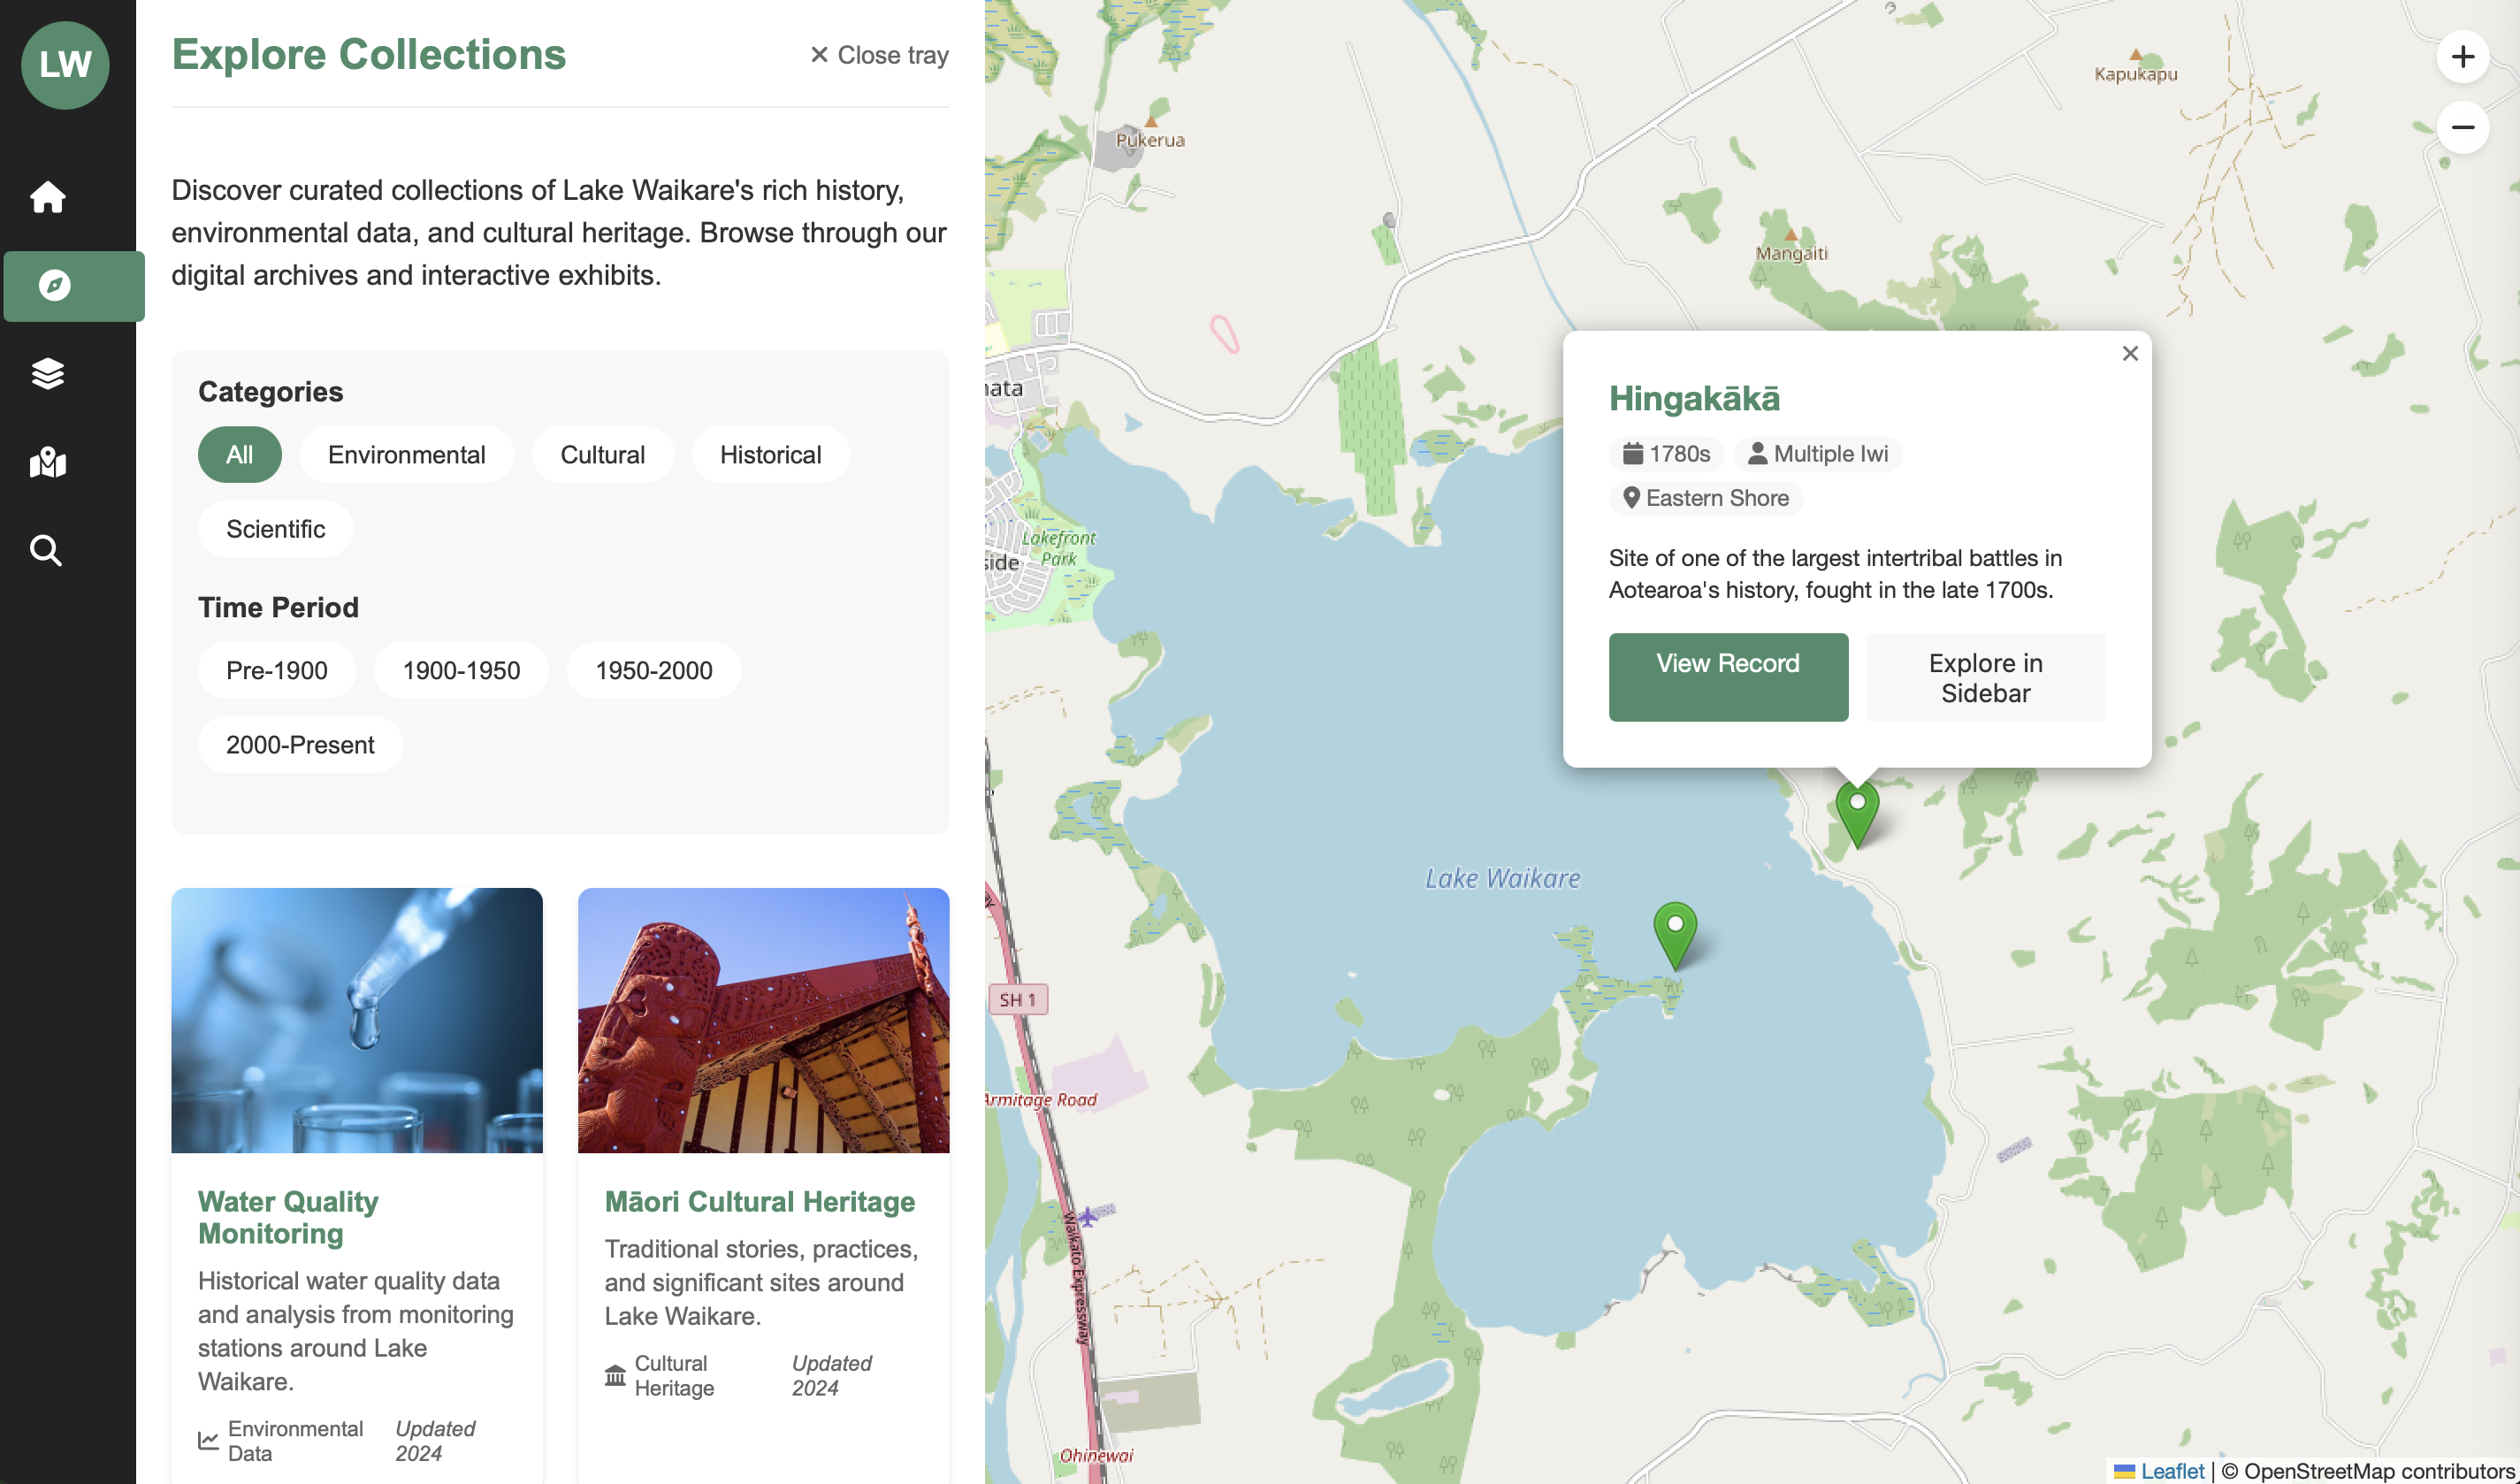
\includegraphics[width=0.8\textwidth]{screenshot/prototype_explore.png}
    \caption{Explore Page}
    \label{fig:architecture}
\end{figure}

The Explore page is designed for users who are interested in discovering content but do not have a specific query in mind. It features a two-column layout: the right side presents an interactive map, while the left side displays a content panel that guides user exploration. The design emphasizes both informational guidance and visual appeal, encouraging users to explore records based on themes and categories.

At the top of the left-hand content panel, introductory text briefly outlines the purpose of the page and creates an immersive atmosphere for browsing. Below this, several category tabs are displayed, allowing users to filter records according to thematic groupings. When a user clicks on a theme, only the records associated with that theme will appear on the map. This structure helps users narrow down what they're viewing and offers a structured way to navigate cultural content—especially useful for open-ended exploration.

Beneath the thematic categories, a timeline-based filter allows users to browse records by historical period, providing a chronological perspective on cultural developments. In addition, to enhance the sense of authenticity and improve visual engagement, theme-related images and short descriptions have been added to some of the categories. These enhancements make the topics more recognizable and help users quickly grasp the cultural background associated with each theme.

Compared to the earlier version, the most significant improvement is that users can now click on records directly from the map to access detailed content pages. This deepens the exploratory experience, allowing users not only to browse thematically but also to dig into the stories and context behind each record. The addition of representative images on the left panel also reinforces the credibility and authenticity of the content, aligning with the project's emphasis on culturally respectful presentation.

By centering the map as the main medium and complementing it with categorized visuals and textual prompts, the Explore page offers an intuitive and layered platform for discovery. Its design promotes interactivity, discoverability, and immersion—making it one of the most engaging interfaces in the system for sparking user curiosity and participation.

\subsection*{4.2.3 Map Layers Page}
\addcontentsline{toc}{subsubsection}{4.2.3 Map Layers Page}
\begin{figure}[H]
    \centering
    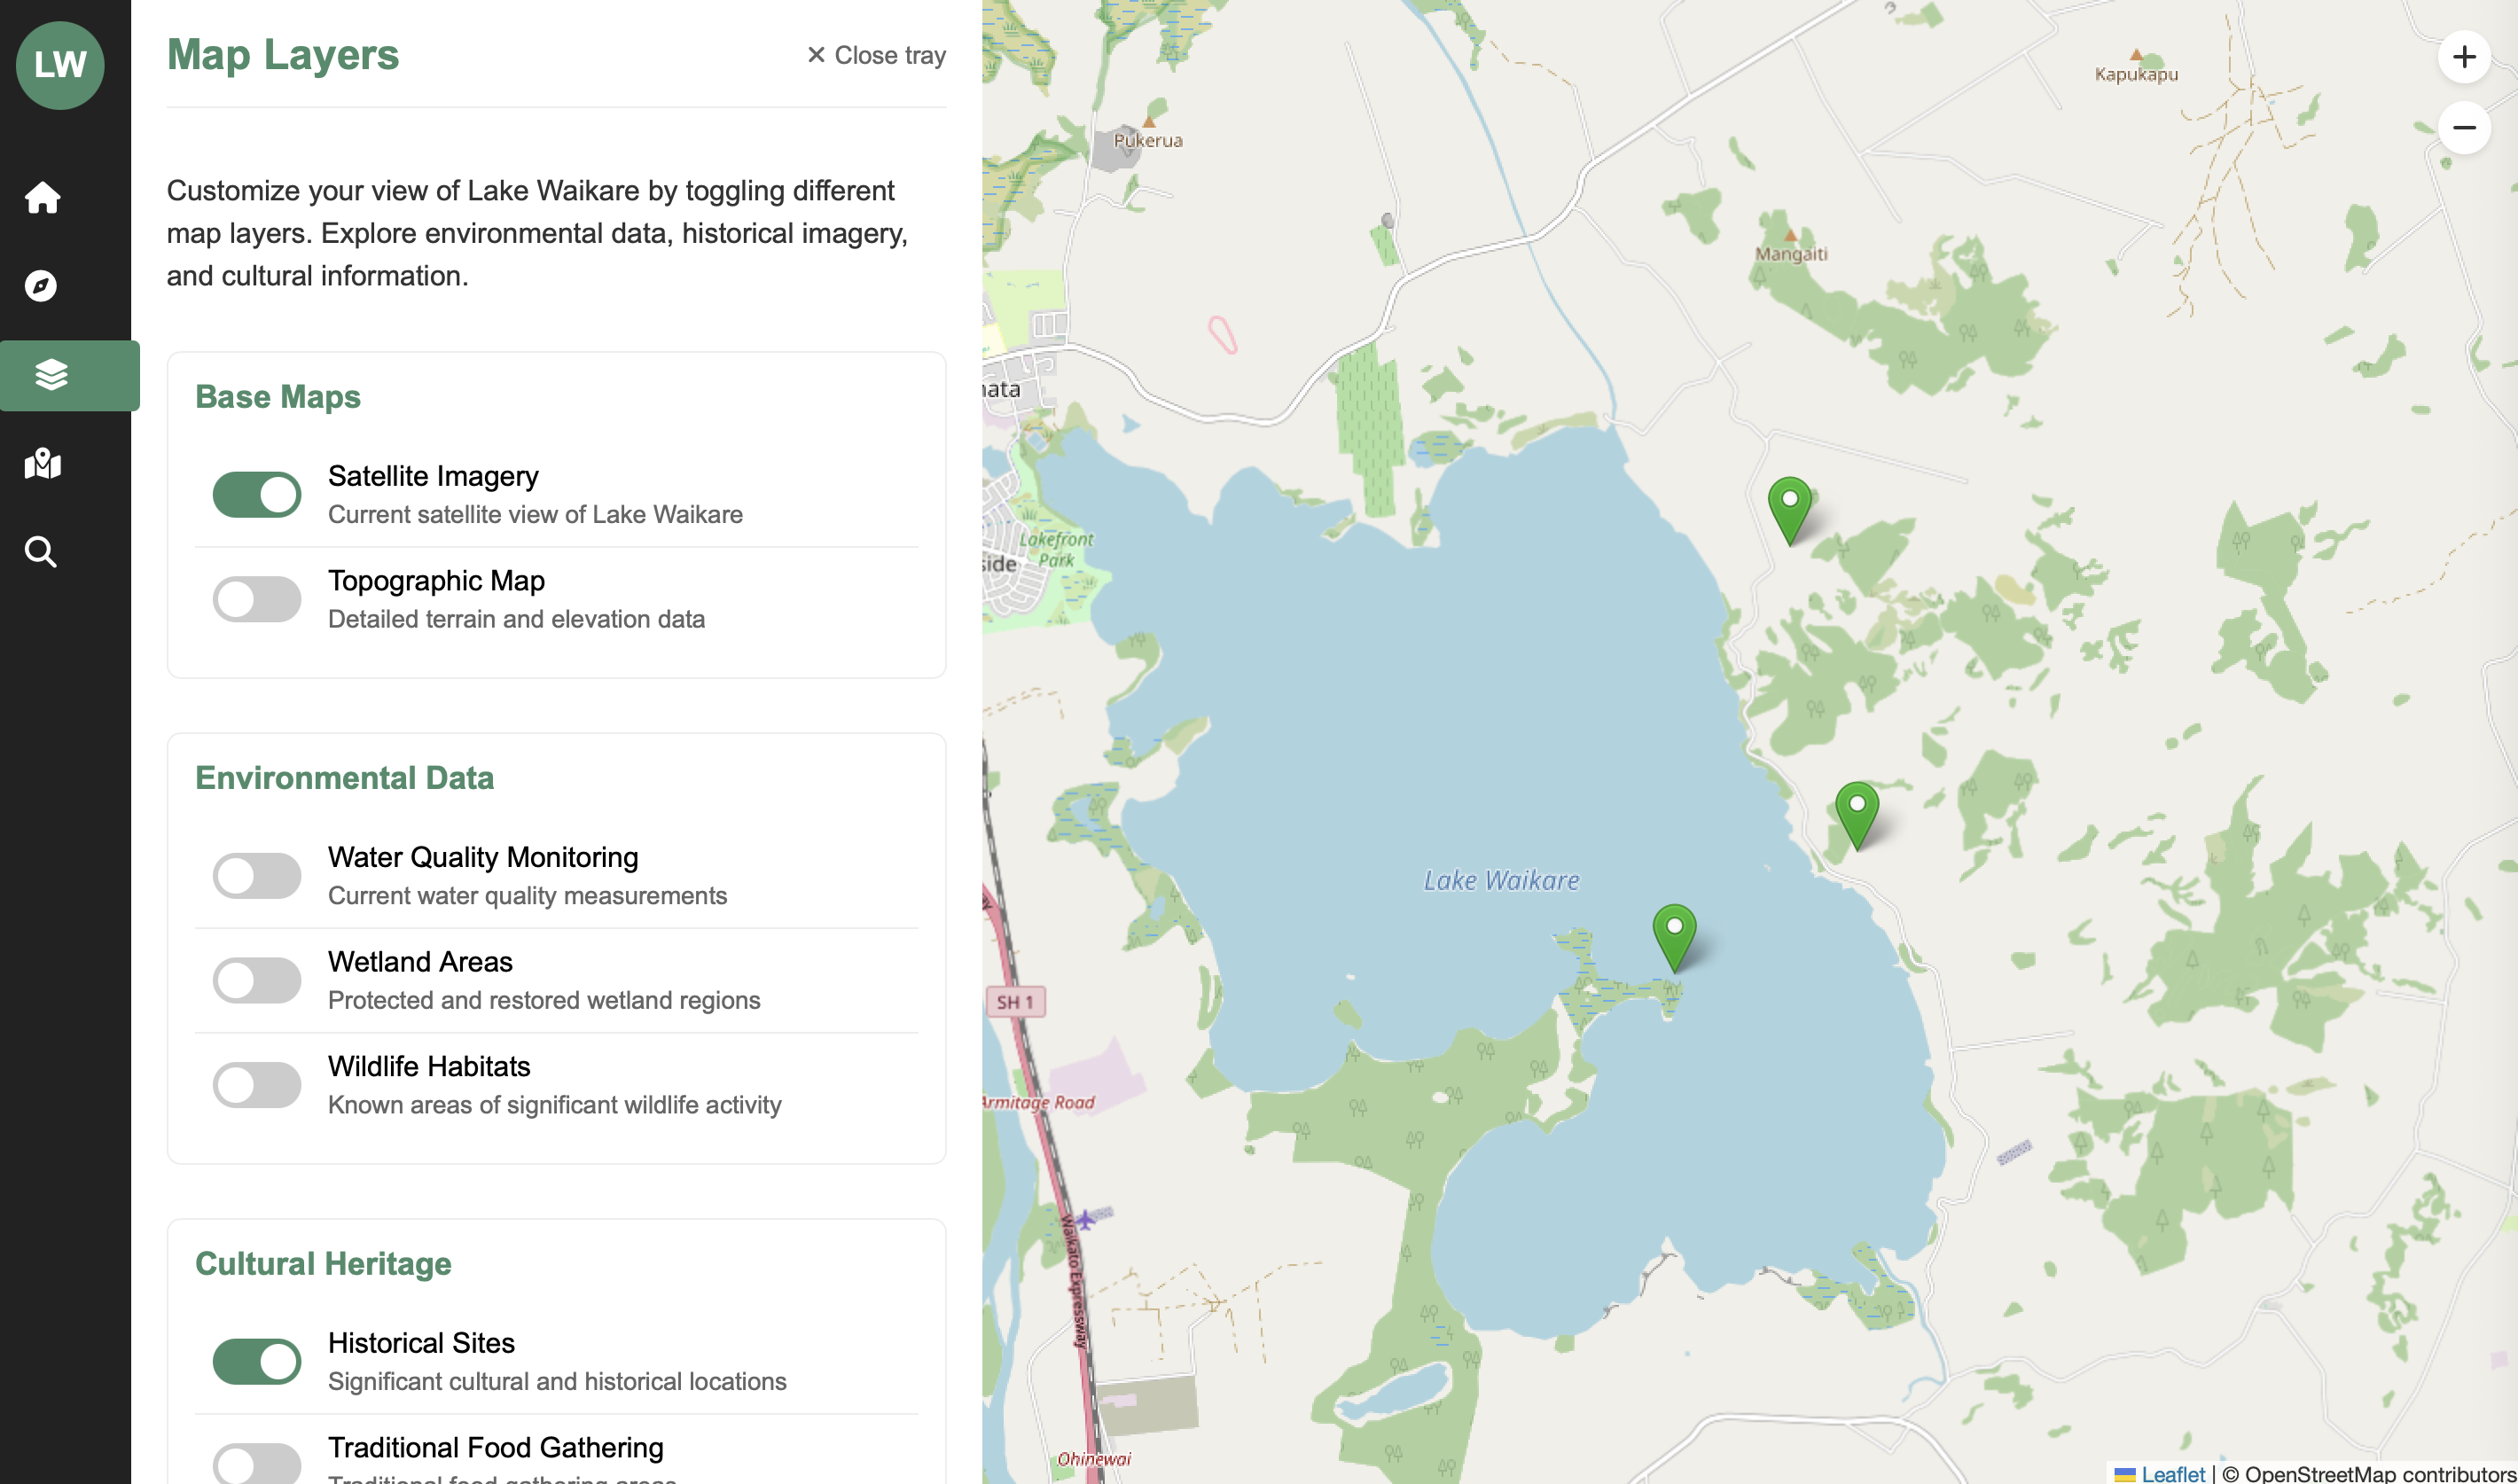
\includegraphics[width=0.8\textwidth]{screenshot/prototype_overlay.png}
    \caption{Overlays Page}
    \label{fig:architecture}
\end{figure}

The Layers Page plays a crucial role in helping users gain a deeper understanding of the map data. By organizing layers into clear categories, the page allows users to flexibly select the data views they need, enhancing the interactivity and multidimensional presentation of the map information.

The overall layout adopts a two-column design, with the layer control panel on the left and a dynamic map display on the right. The control panel categorizes all layers into three primary groups: Cultural Heritage, Environmental Data, and Historical Data. This classification is based on an in-depth analysis of the project's content themes, aiming to help users quickly identify and filter the data categories of interest. Each category is presented as a card, visually distinct and easy to browse and operate.

Functionally, each layer is equipped with a toggle switch in the panel, allowing users to show or hide the corresponding layer on the map. When activated, the switch highlights to clearly indicate the layer is active; when deactivated, it remains white, signaling that the layer is hidden. This design not only improves user experience but also ensures immediate feedback, enabling users to observe map changes in real-time.

Additionally, the map area dynamically updates according to the selected layers and supports multiple layers being displayed simultaneously for comprehensive analysis. For example, when users select multiple layers from both the Cultural Heritage and Environmental Data categories, the map overlays these data to reveal spatial relationships and interactions between different datasets.

In this version, two new base map layers have been added: Satellite Imagery and Topographic Map. These base layers provide richer geographic context, adding depth and realism to the map display. Users can freely switch between these two base maps to choose the most suitable view for different analytical scenarios.

Compared to earlier versions, the current design strengthens the logical classification and visual hierarchy of layers and optimizes the interaction flow for smoother and more natural user operations. The addition of card-style categories and toggle switches significantly improves the convenience and efficiency of map layer management, while the new base layers greatly enrich the map's expressiveness.

In summary, the Layers Page enhances users' ability to explore map data through a scientific classification system and flexible interaction design. This page not only offers a clear interface for managing layers but also serves as a key bridge within the overall information architecture, supporting users to delve deeper into the rich cultural and environmental information behind the project.

\subsection*{4.2.4 Map View Page}
\addcontentsline{toc}{subsubsection}{4.2.4 Map View Page}
\begin{figure}[H]
    \centering
    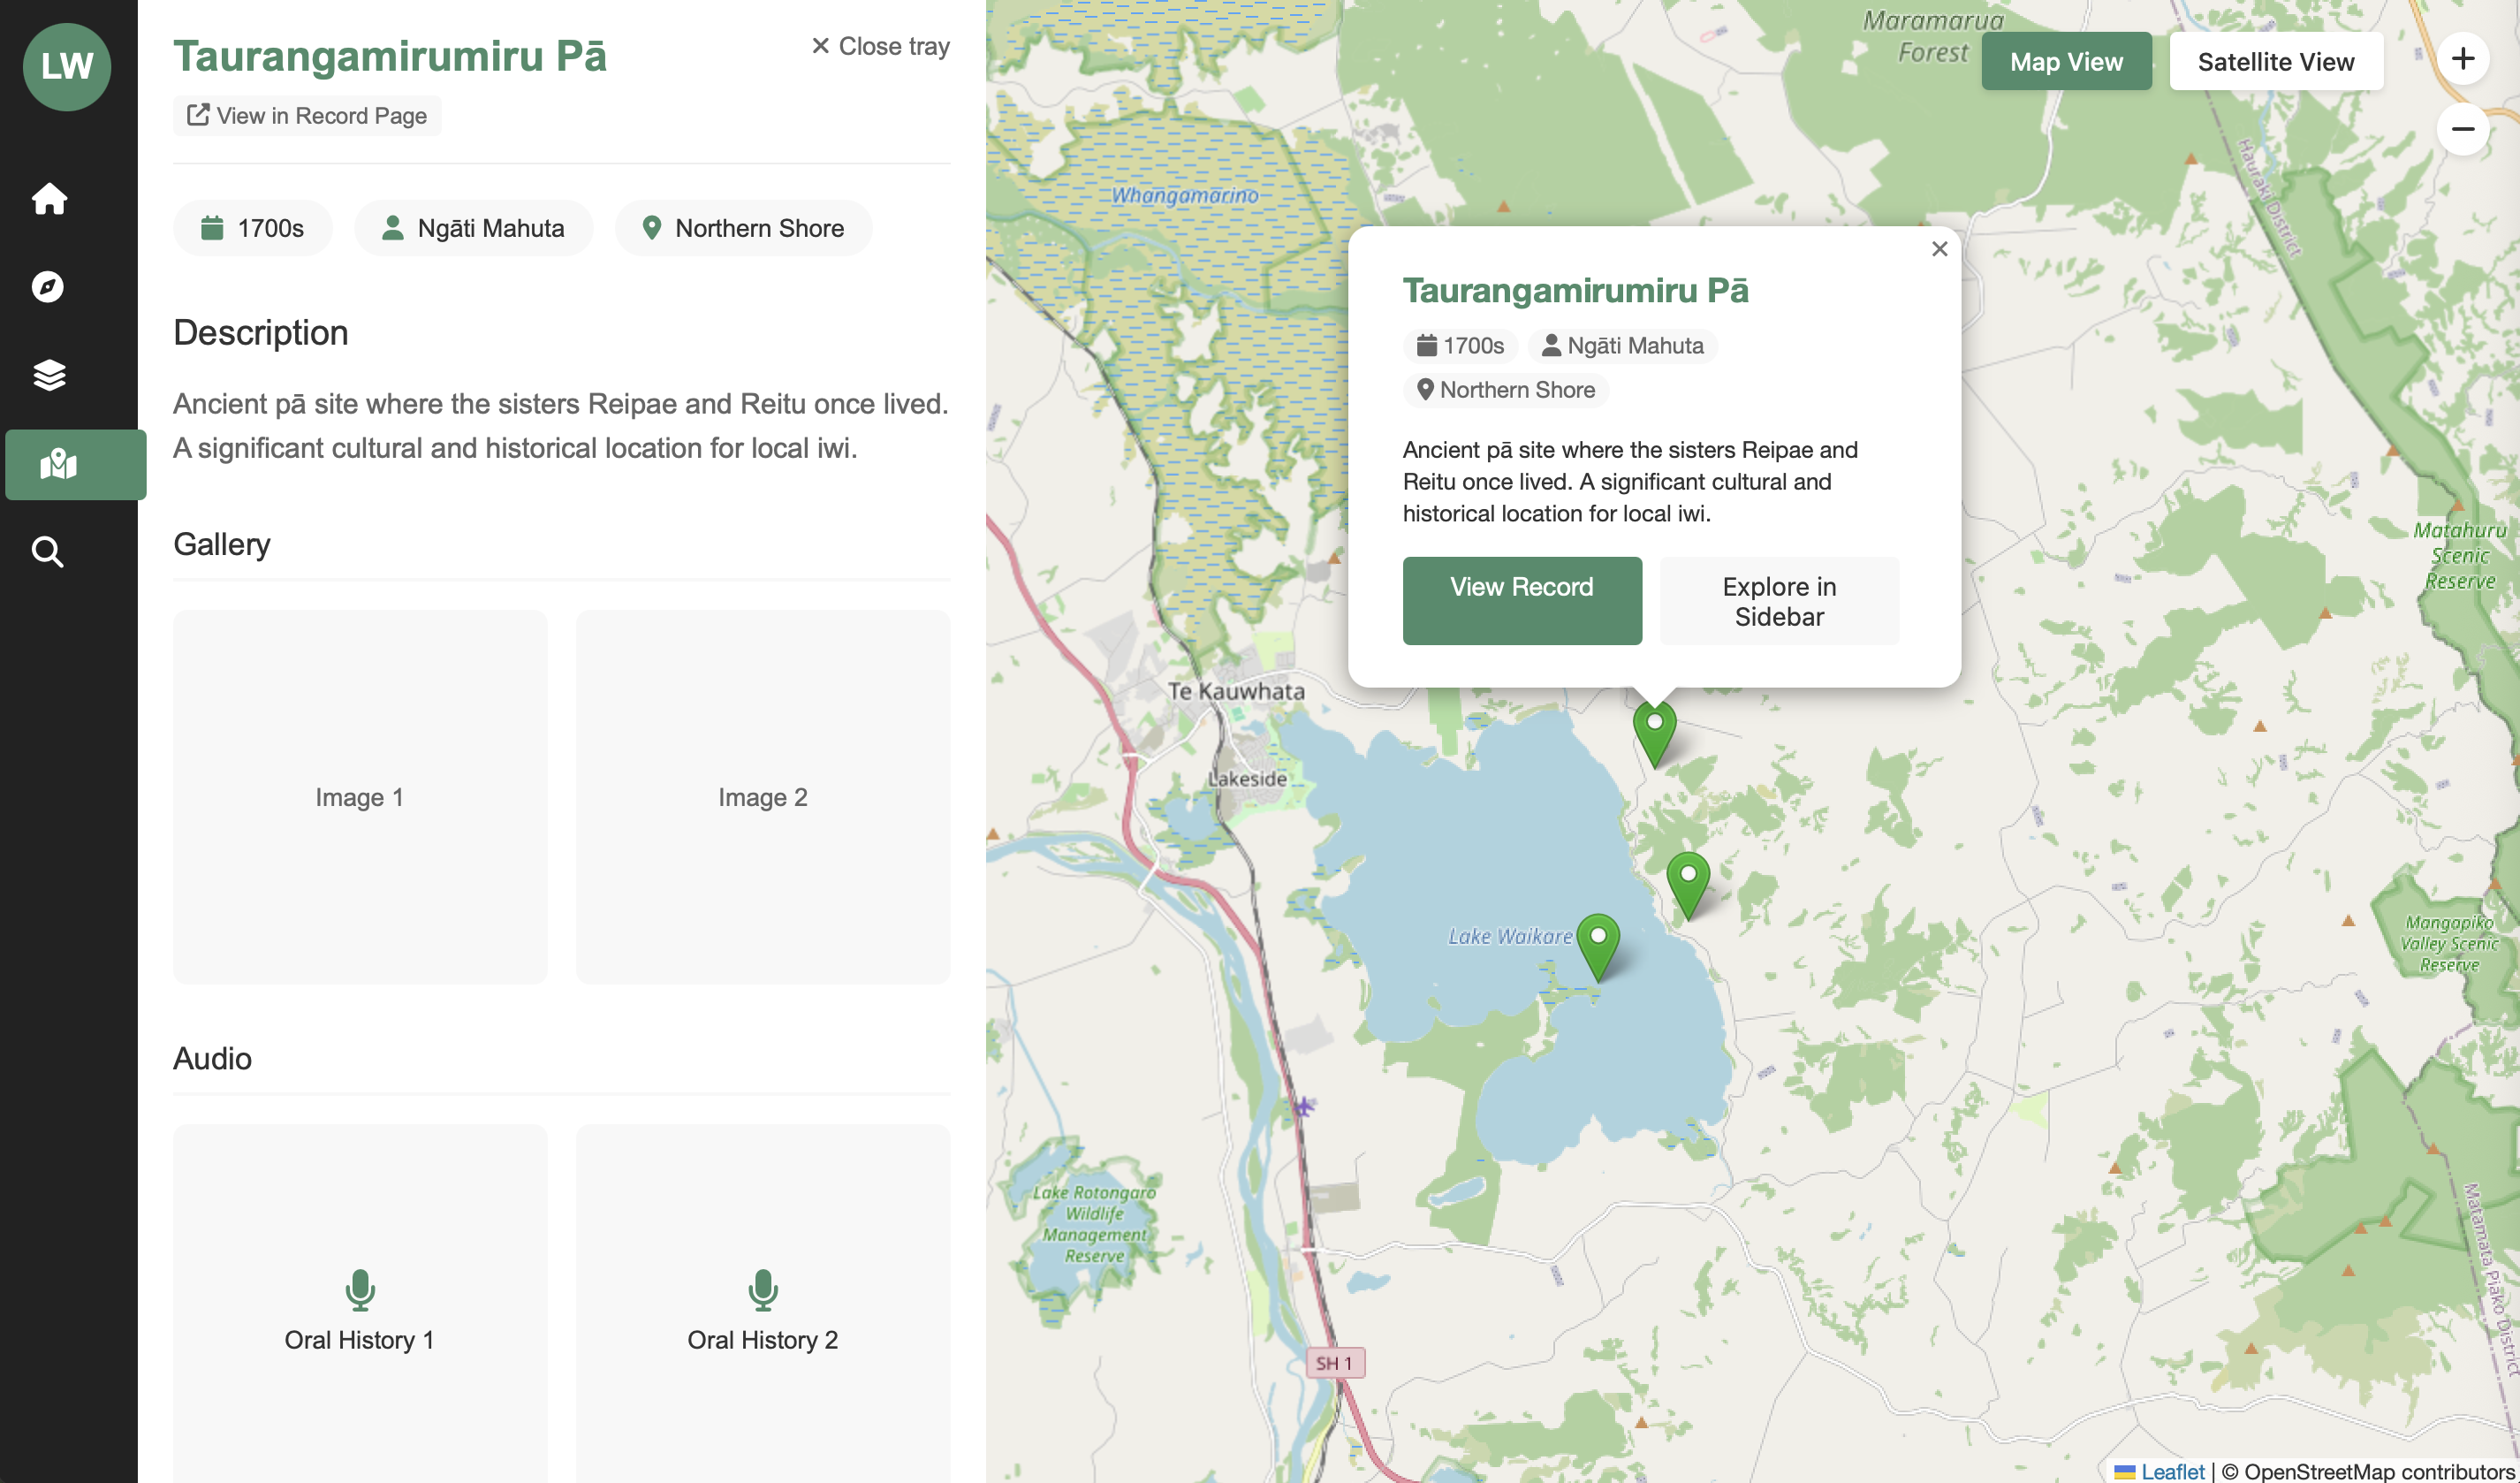
\includegraphics[width=0.8\textwidth]{screenshot/prototype_mapview.png}
    \caption{Map View Page}
    \label{fig:architecture}
\end{figure}

The Map View page can be accessed either through the "Explore Map" button on the Home page or via the navigation buttons in the left sidebar, allowing users to seamlessly enter the map interface from different contexts. This flexibility ensures that both first-time visitors and returning users can easily navigate to and engage with the core features of the application.

The main content of this page is a map centered on Lake Waikare, marked with multiple pins. Each pin represents a specific record. When a pin is clicked, a popup appears, displaying a concise summary of the record, including an overview, geographical and temporal details, and links to related resources. Users can click through to view the full record, making it easy to explore content in depth based on their interests.

In this version, the Map View introduces two new base map layers: satellite imagery and a standard topographic map. Users can freely switch between these map modes to gain a richer geographical perspective of the area. This feature enhances both visual clarity and contextual understanding of the environment. The map also supports zooming in and out, giving users precise control over the area they wish to explore, from wide overviews to specific local details.

From an interaction standpoint, the update goes beyond traditional popups by introducing the "Explore in Sidebar" feature. When a marker is clicked, the related record details are also displayed in the content panel on the right-hand side of the map. This enables users to browse the record information without leaving the map interface, significantly improving usability and engagement. The dual display—popup and sidebar—streamlines navigation and supports multitasking and comparative analysis.

Overall, the Map View page focuses on a clean design and practical functionality. By combining multiple map layers and enriched interactive features, it serves as the central entry point to the application's data space. As one of the core features of the application, the Map View bridges geographical data with cultural and historical records, allowing users to gain multi-dimensional insight into the Lake Waikare area. This reinforces the educational value of the platform and enhances user experience through intuitive, immersive exploration.

\subsection*{4.2.5 Search Page}
\addcontentsline{toc}{subsubsection}{4.2.5 Search Page}
\begin{figure}[H]
    \centering
    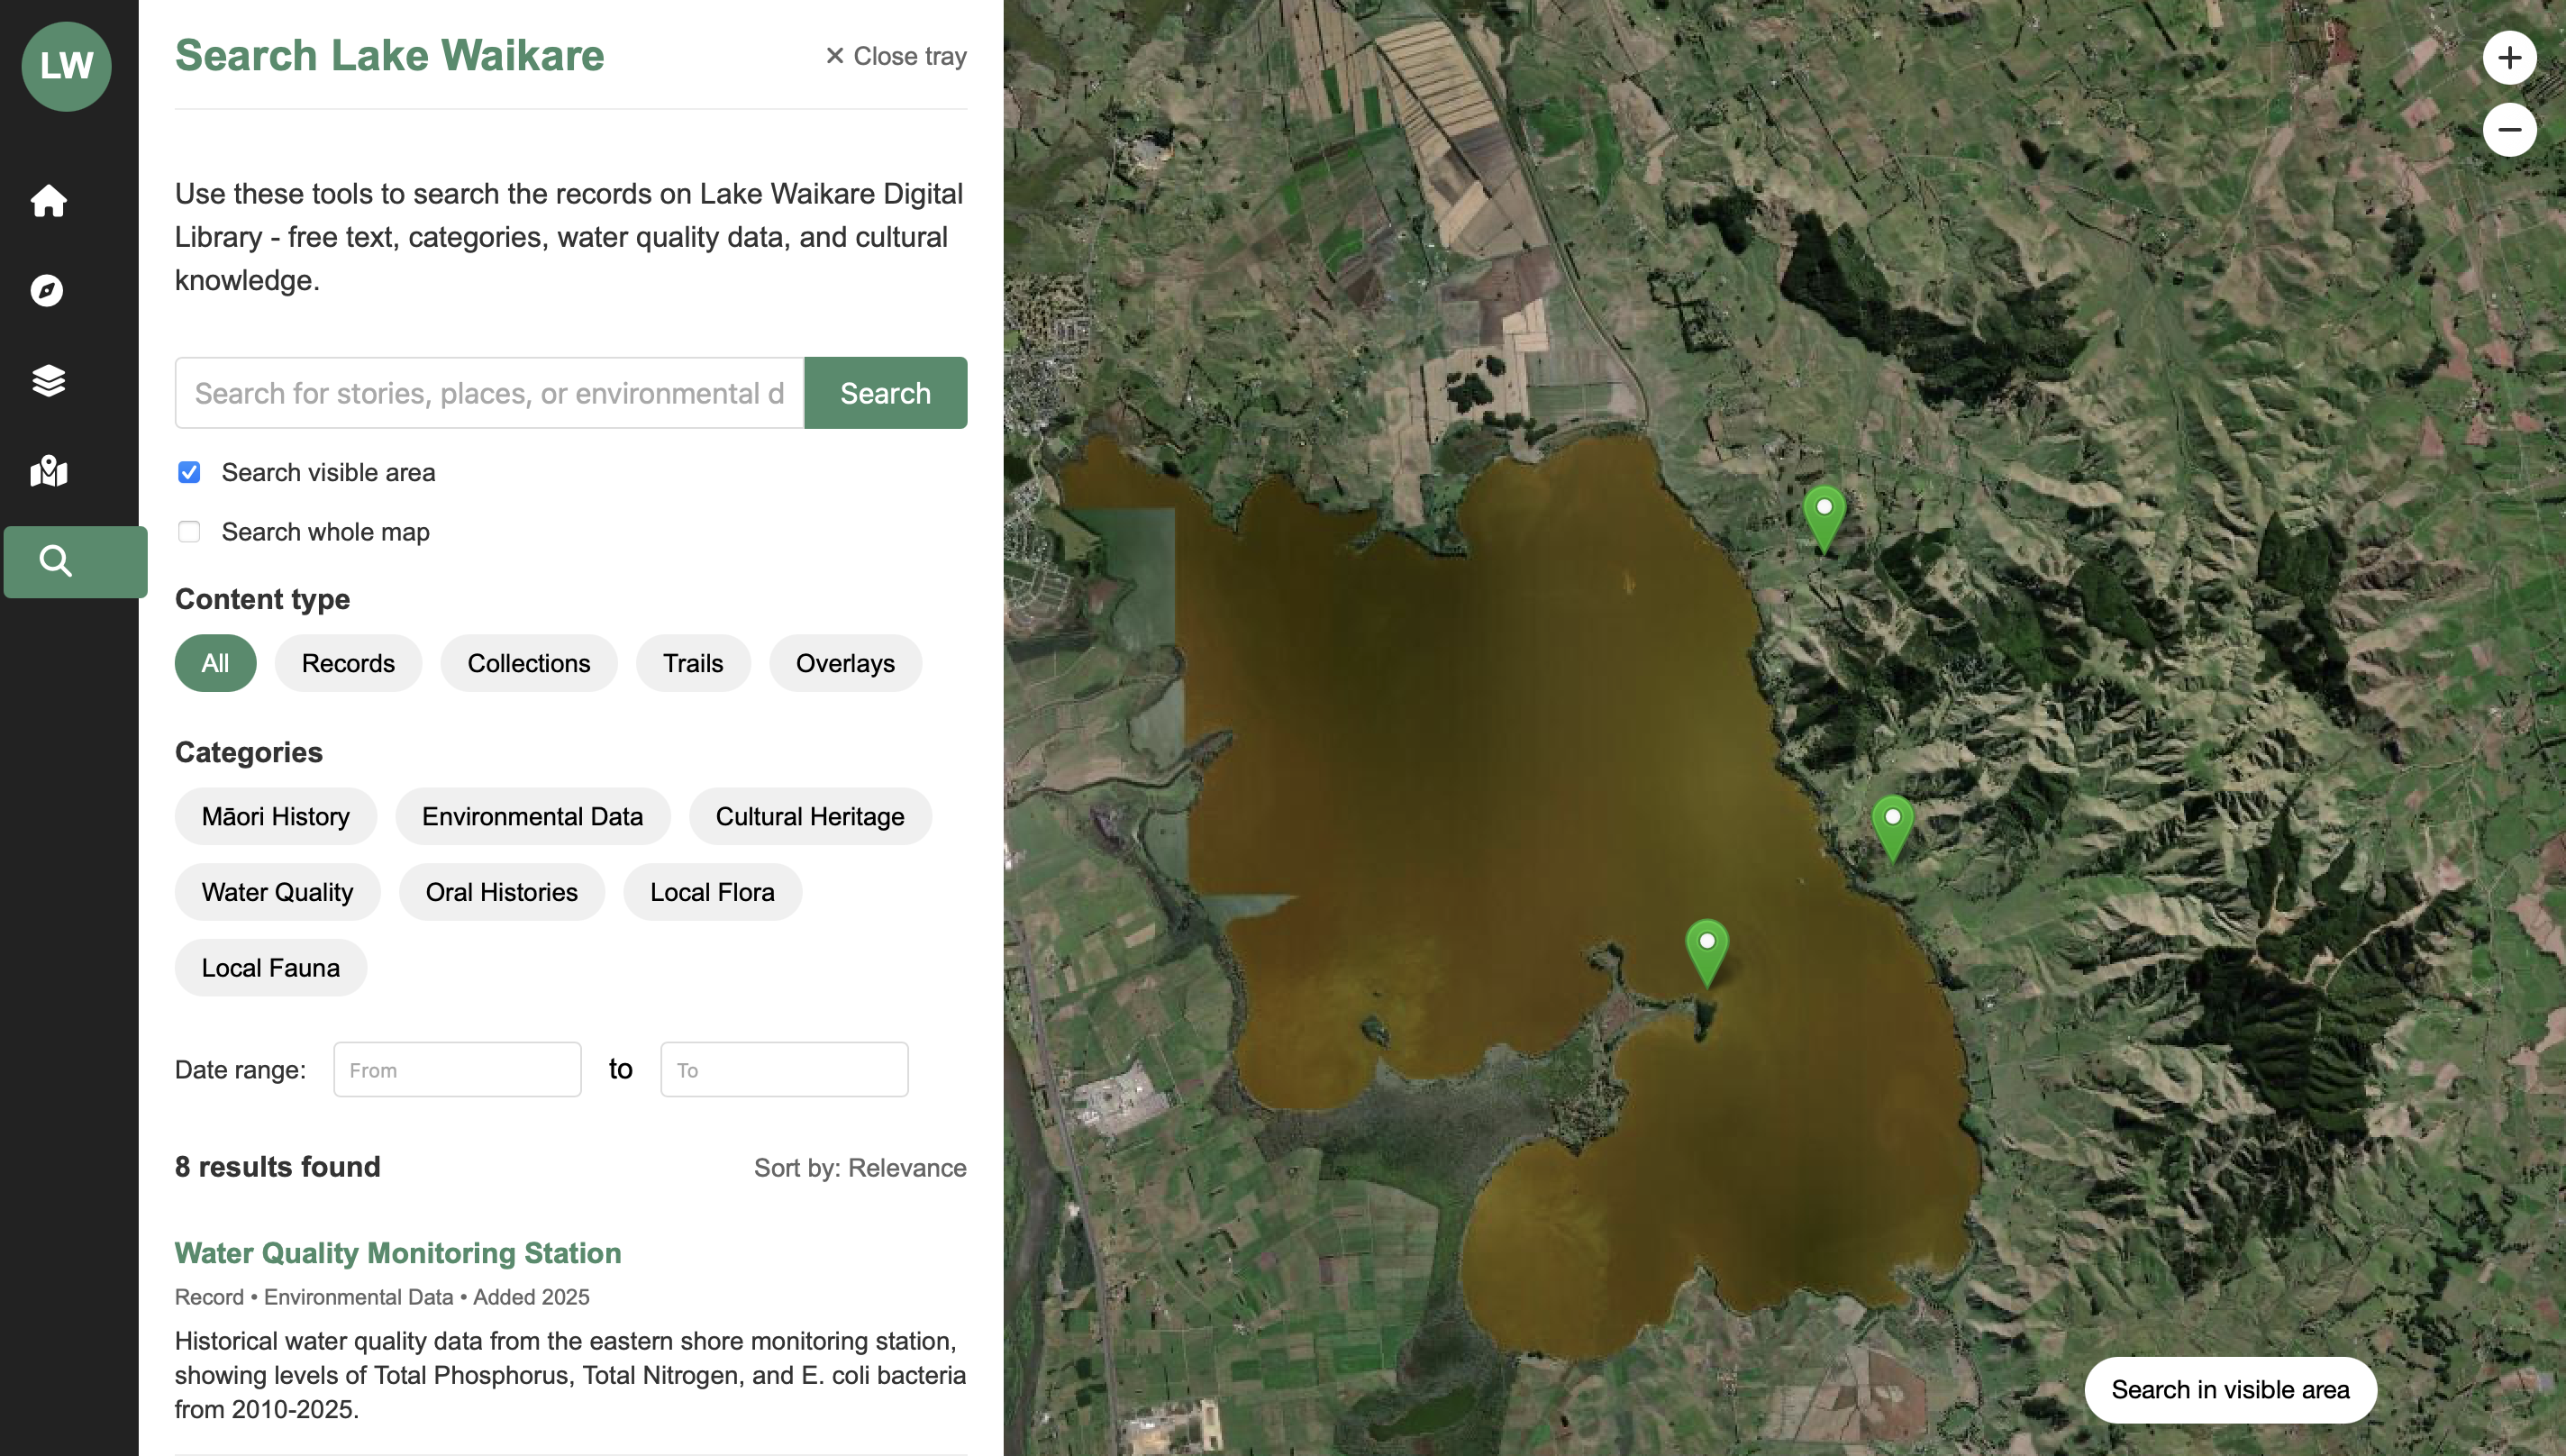
\includegraphics[width=0.8\textwidth]{screenshot/prototype_search.png}
    \caption{Search Page}
    \label{fig:architecture}
\end{figure}

The main search interface is located on the left side of the page, with a search bar at the top of the sidebar. The placeholder text reads "Search stories, places…" Users can enter keywords or place names to quickly find relevant content. The search bar is designed to be simple and intuitive, supporting fuzzy matching and multiple keyword combinations to help users efficiently locate the information they need.

Below the search bar is a toggle control labeled "Search visible area / Search whole map," which controls whether the search scope syncs with the current map view. When turned on, search results are limited to data within the visible map area; when off, the search queries the entire map dataset. This feature enhances flexibility, allowing users to search either within a local area or across the entire map.

Users can further refine their search results by selecting one of five content types (All, Records, Collections, Trails, or Overlays) and one or more category tags (e.g., Māori History or Environmental Data). This multi-dimensional filtering enables users to quickly narrow down results and accurately pinpoint content of interest, significantly improving search efficiency.

The page also offers a date range selector, allowing users to restrict search results to a specific time period—ideal for exploring historical events or environmental monitoring data. After setting the filters, users click Search, and matching results gradually load into the results display area on the left. The displayed content includes text, images, videos, and map markers, supporting a multi-faceted understanding of the results.

Overall, the Search Page serves as a core function for quickly locating information. Through rich filtering options and flexible scope controls, it helps users efficiently extract needed content from large and complex datasets. Whether for casual browsing or professional research, this page provides a convenient and precise retrieval channel, greatly enhancing system usability and user experience.

\subsection*{4.2.6 Child Mode}
\addcontentsline{toc}{subsubsection}{4.2.6 Child Mode}
\begin{figure}[H]
    \centering
    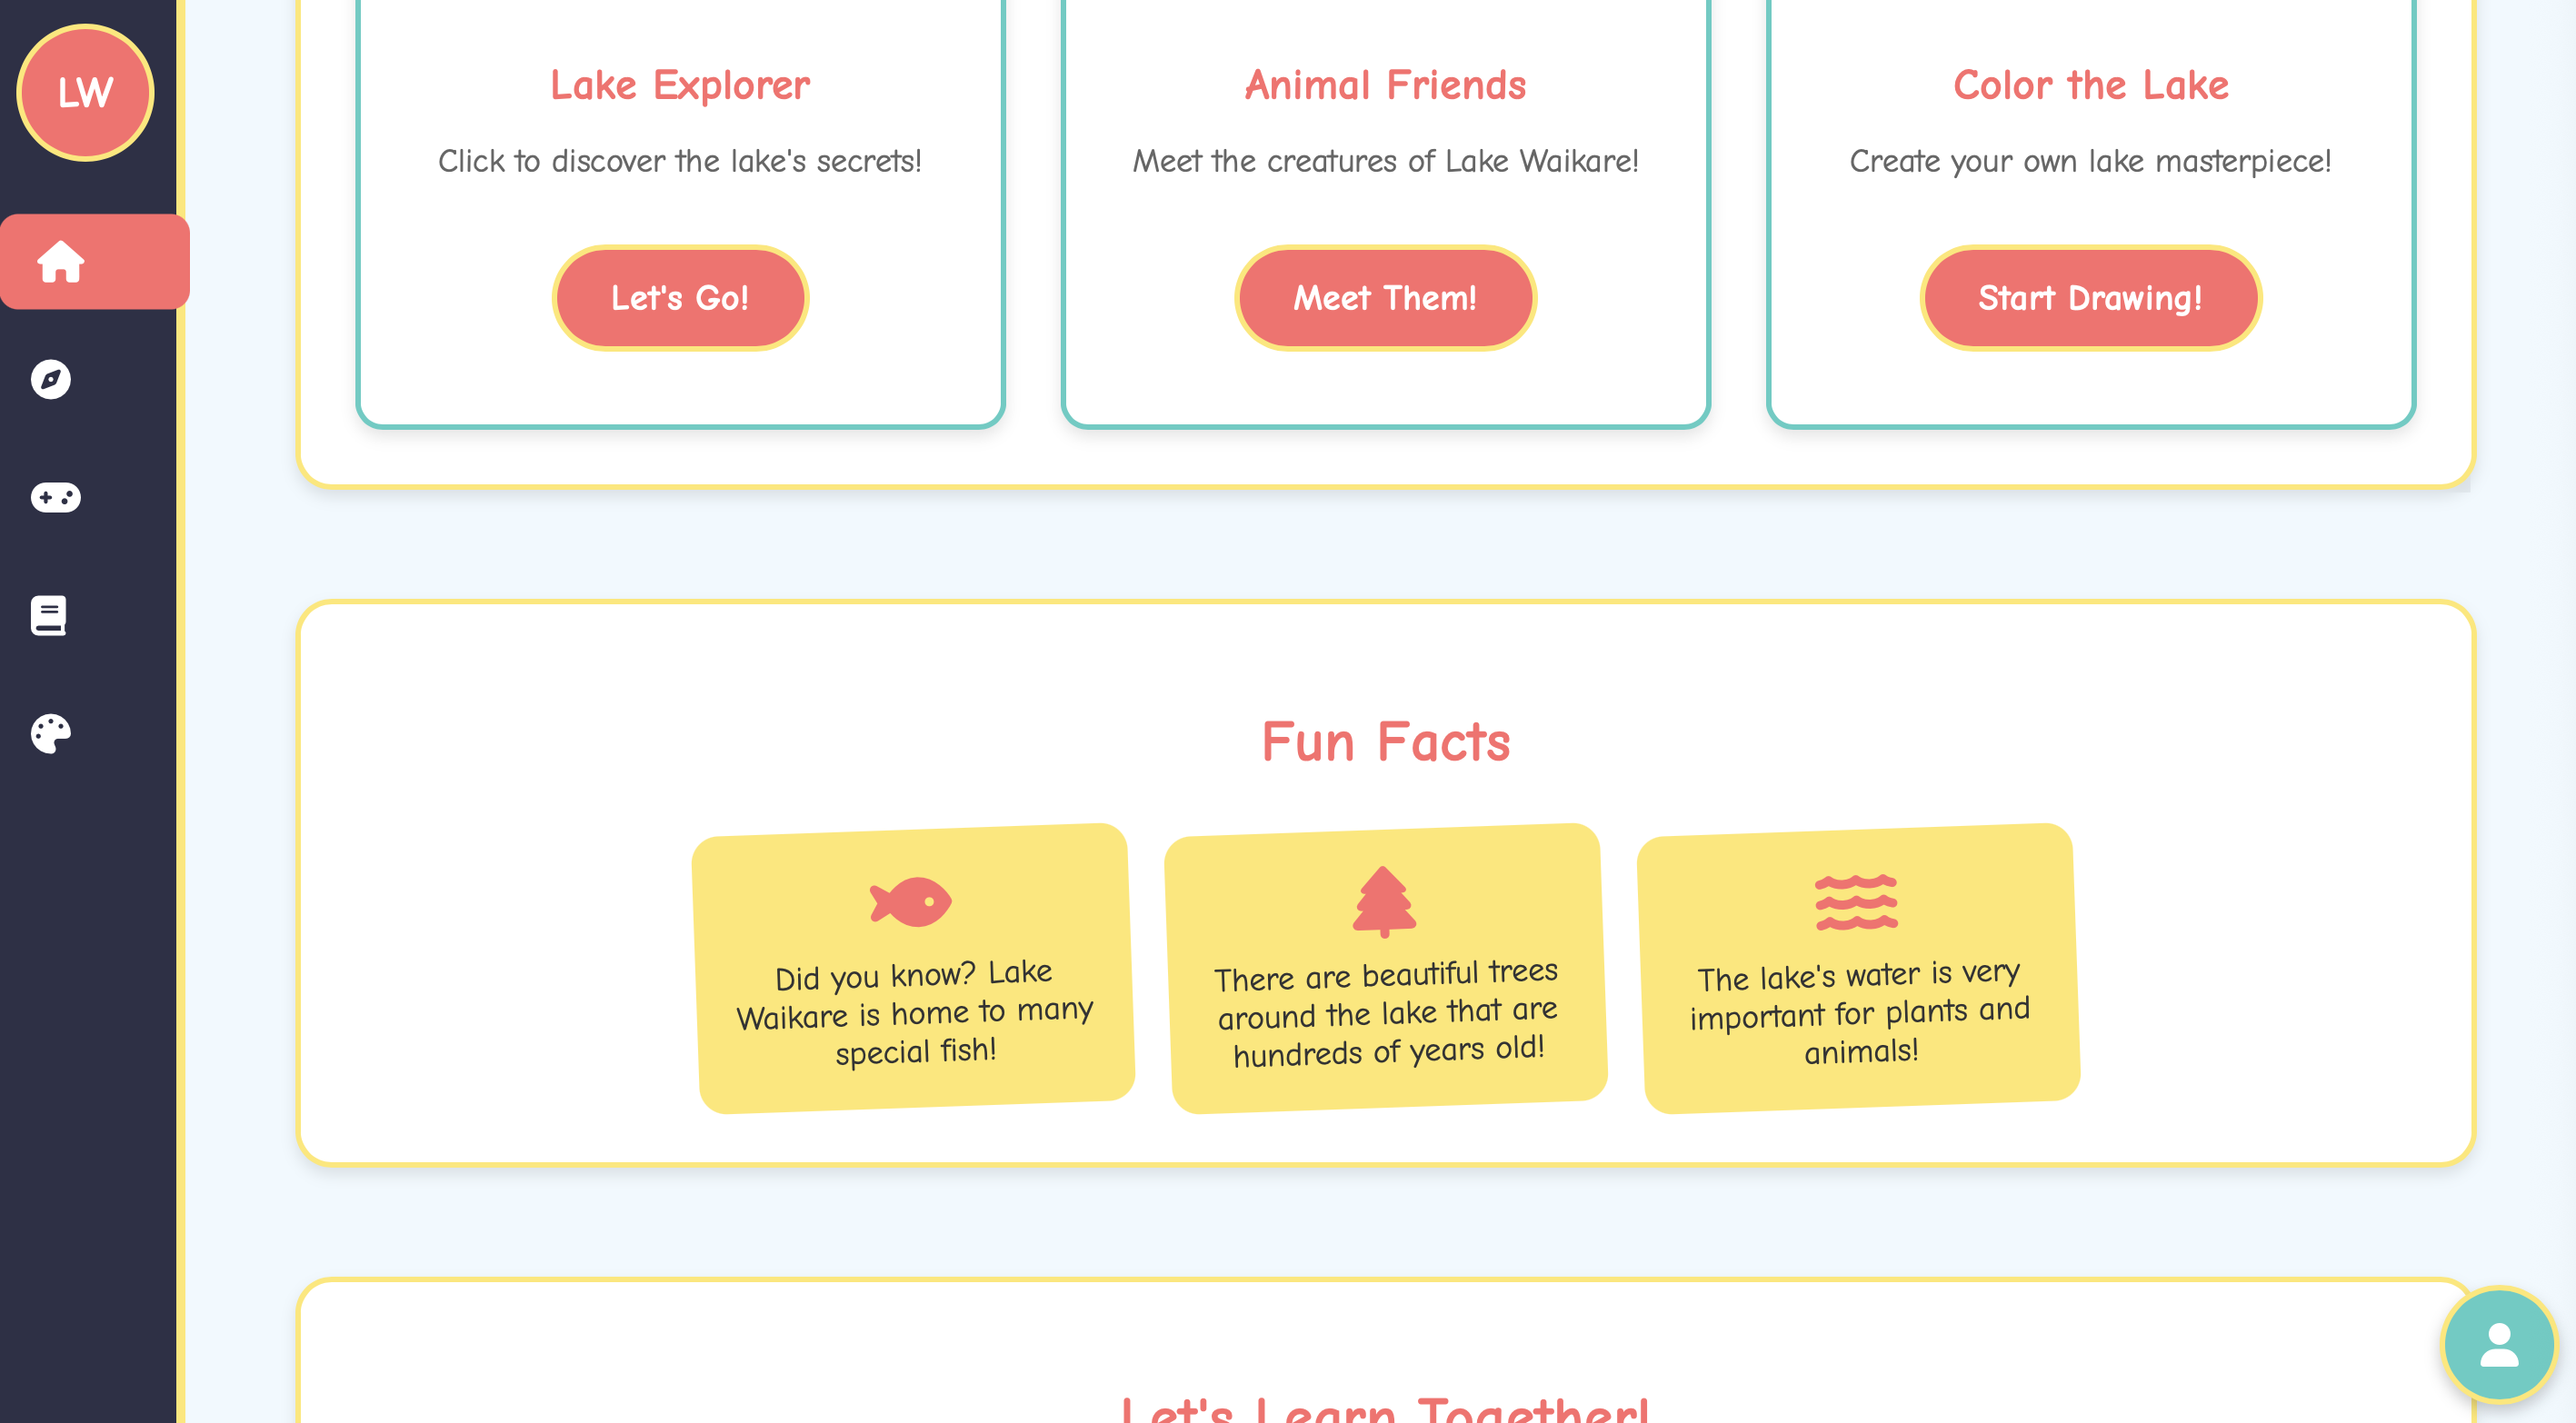
\includegraphics[width=0.8\textwidth]{screenshot/prototype_childmode.png}
    \caption{Child Mode}
    \label{fig:architecture}
\end{figure}

Child Mode is designed to provide children with a fun, safe, and age-appropriate environment to interact with the content, encouraging exploration and learning of Māori culture through a child-friendly approach. The interface features simplified navigation with large buttons, minimal text, and bright, high-contrast colors that match children's interaction patterns, making the website easy to use.

A key aspect of this mode is the inclusion of creative interactive features and visual effects, such as animations, cartoon-style icons, and simple games. These enhancements aim to boost children's interest and motivation to engage with Māori culture.

Additionally, the prototype plans to add diverse activities like map exploration, stories, games, and coloring to further increase children's engagement. These activities provide a more immersive and enjoyable learning experience, encouraging children to explore cultural content in a playful and educational manner.

To support focused and age-appropriate learning, the website filters out complex or unsuitable content for younger users. By attracting more children to the platform, the project helps pass cultural knowledge on to the next generation.

Child Mode can be activated via a floating button located at the bottom-right corner of the home page, displayed as a clear cartoon-style icon. Hovering over the icon reveals a tooltip explaining its function. While in Child Mode, users can switch back to Normal Mode by clicking the same floating button.

On the Child Mode home page, activities and stories are presented using a card-style layout that aligns with children's reading habits, helping them quickly find their favorite content. Each activity or story page features carefully selected high-quality content enhanced with images and audio narration to support users who may not yet be proficient in reading or writing.

Overall, the platform aims to make historical and cultural content accessible and enjoyable for all users. Beyond entertainment and education for children, the website also serves as a valuable tool for early family education and a complementary resource for Māori cultural education in schools.

Child Mode is designed with a focus on usability, engagement, safety, and cultural authenticity.

\subsection*{4.2.7 Browse Records Page}
\addcontentsline{toc}{subsubsection}{4.2.7 Browse Records Page}
\begin{figure}[H]
    \centering
    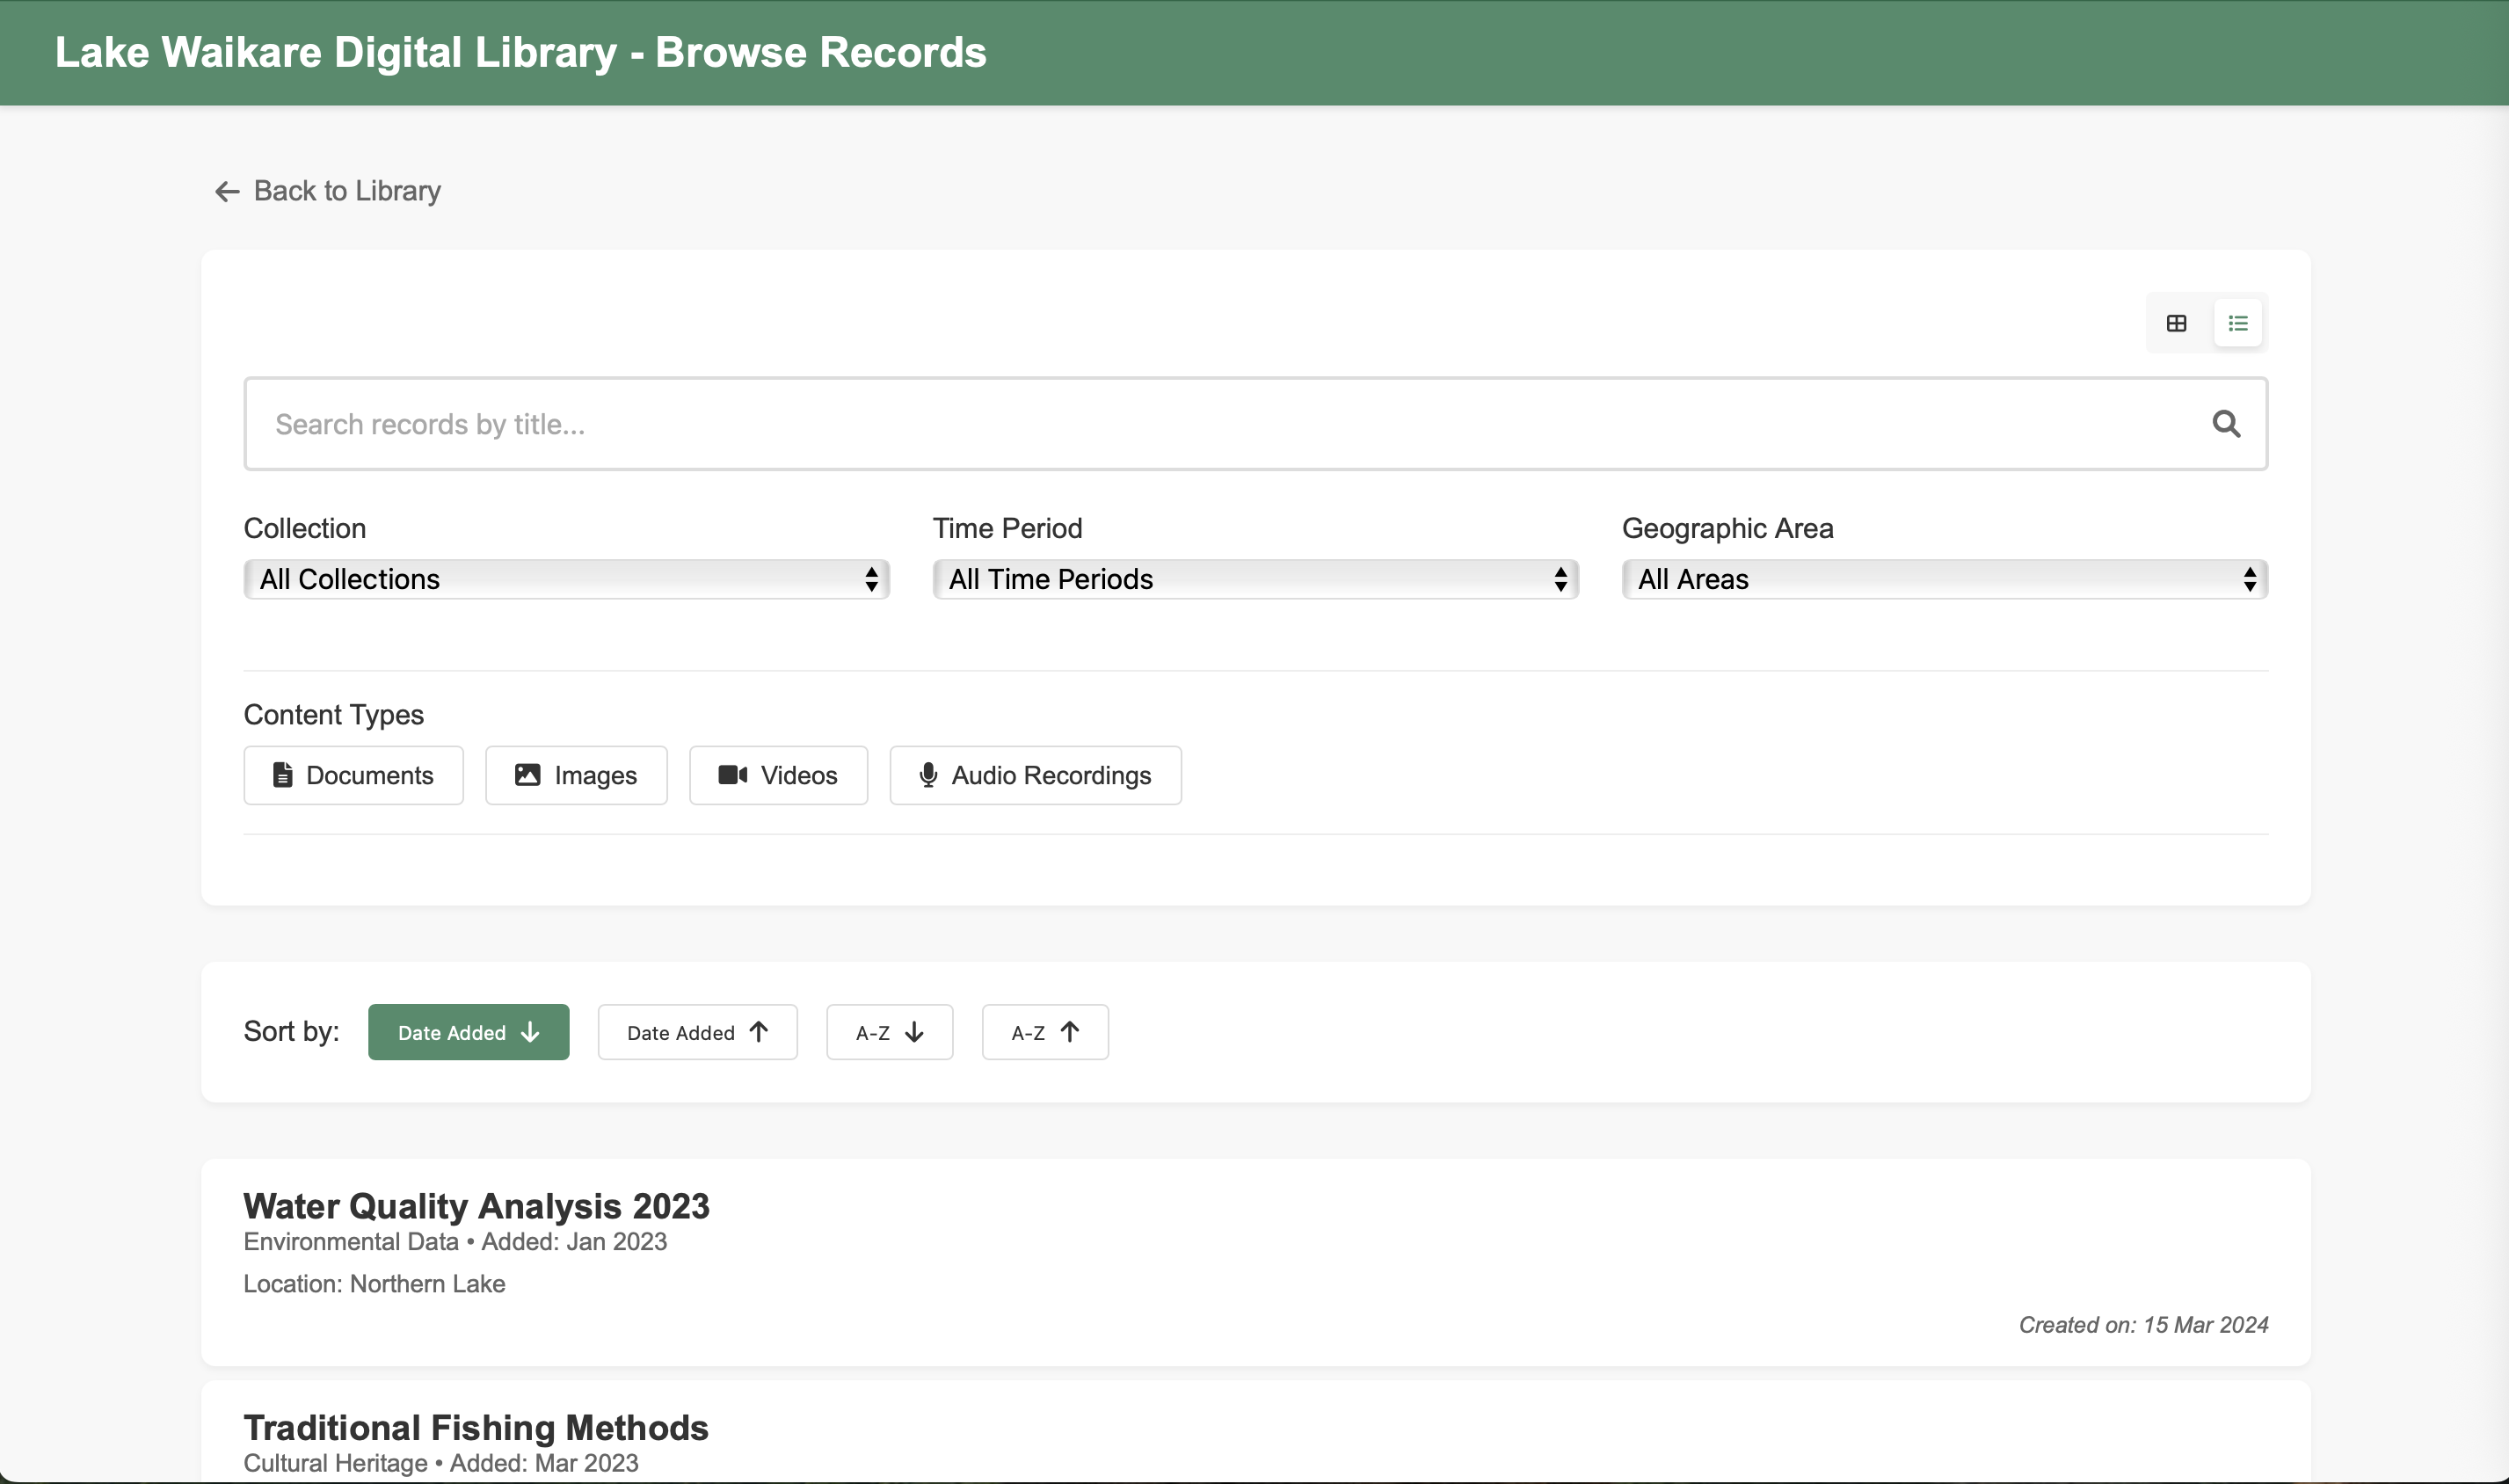
\includegraphics[width=0.8\textwidth]{screenshot/prototype_records.png}
    \caption{Records Page}
    \label{fig:architecture}
\end{figure}

The Browse Records page serves as a vital gateway for users to deeply explore the rich and diverse cultural and environmental resources within the project. The design thoughtfully incorporates multi-dimensional filtering and flexible display options to meet the varied needs of different users. At the top of the page lies a comprehensive filtering and display control panel, where users can quickly locate relevant content by entering keywords or place names into the search box, enabling efficient and precise searches.

This filtering panel not only allows users to narrow results by Collections, providing a thematic grouping of data, but also includes filters for Time Period and Geographic Area, helping users refine their queries along temporal and spatial dimensions for more targeted results. Additionally, content type filters (Documents, Images, Videos, Audio Recordings) offer convenient options to isolate materials by media format, catering to various use cases and research interests.

In the upper right corner of the filter panel, a display toggle lets users switch effortlessly between grid and list views, accommodating different browsing habits and reading preferences, thereby enhancing interaction and visual presentation. Just below the filter panel, sorting options are available, allowing users to order results by date added or alphabetical order, facilitating organized and focused content review.

The main body of the page presents all records matching the selected criteria in a clear and structured layout, where each record displays essential information in a concise manner to support quick browsing and selection. By clicking on any record, users are directed to a detailed record page featuring enriched textual descriptions, multimedia resources, and related links, offering a deeper understanding and engagement with the content.

Overall, the Browse Records page combines powerful filtering capabilities, diverse display modes, and smart sorting functions to significantly enhance search efficiency and browsing convenience. This page not only improves user experience but also provides robust technical support and a user-friendly platform for the dissemination and preservation of cultural and environmental information.

\subsection*{4.2.8 Record View Page}
\addcontentsline{toc}{subsubsection}{4.2.8 Record View Page}
\begin{figure}[H]
    \centering
    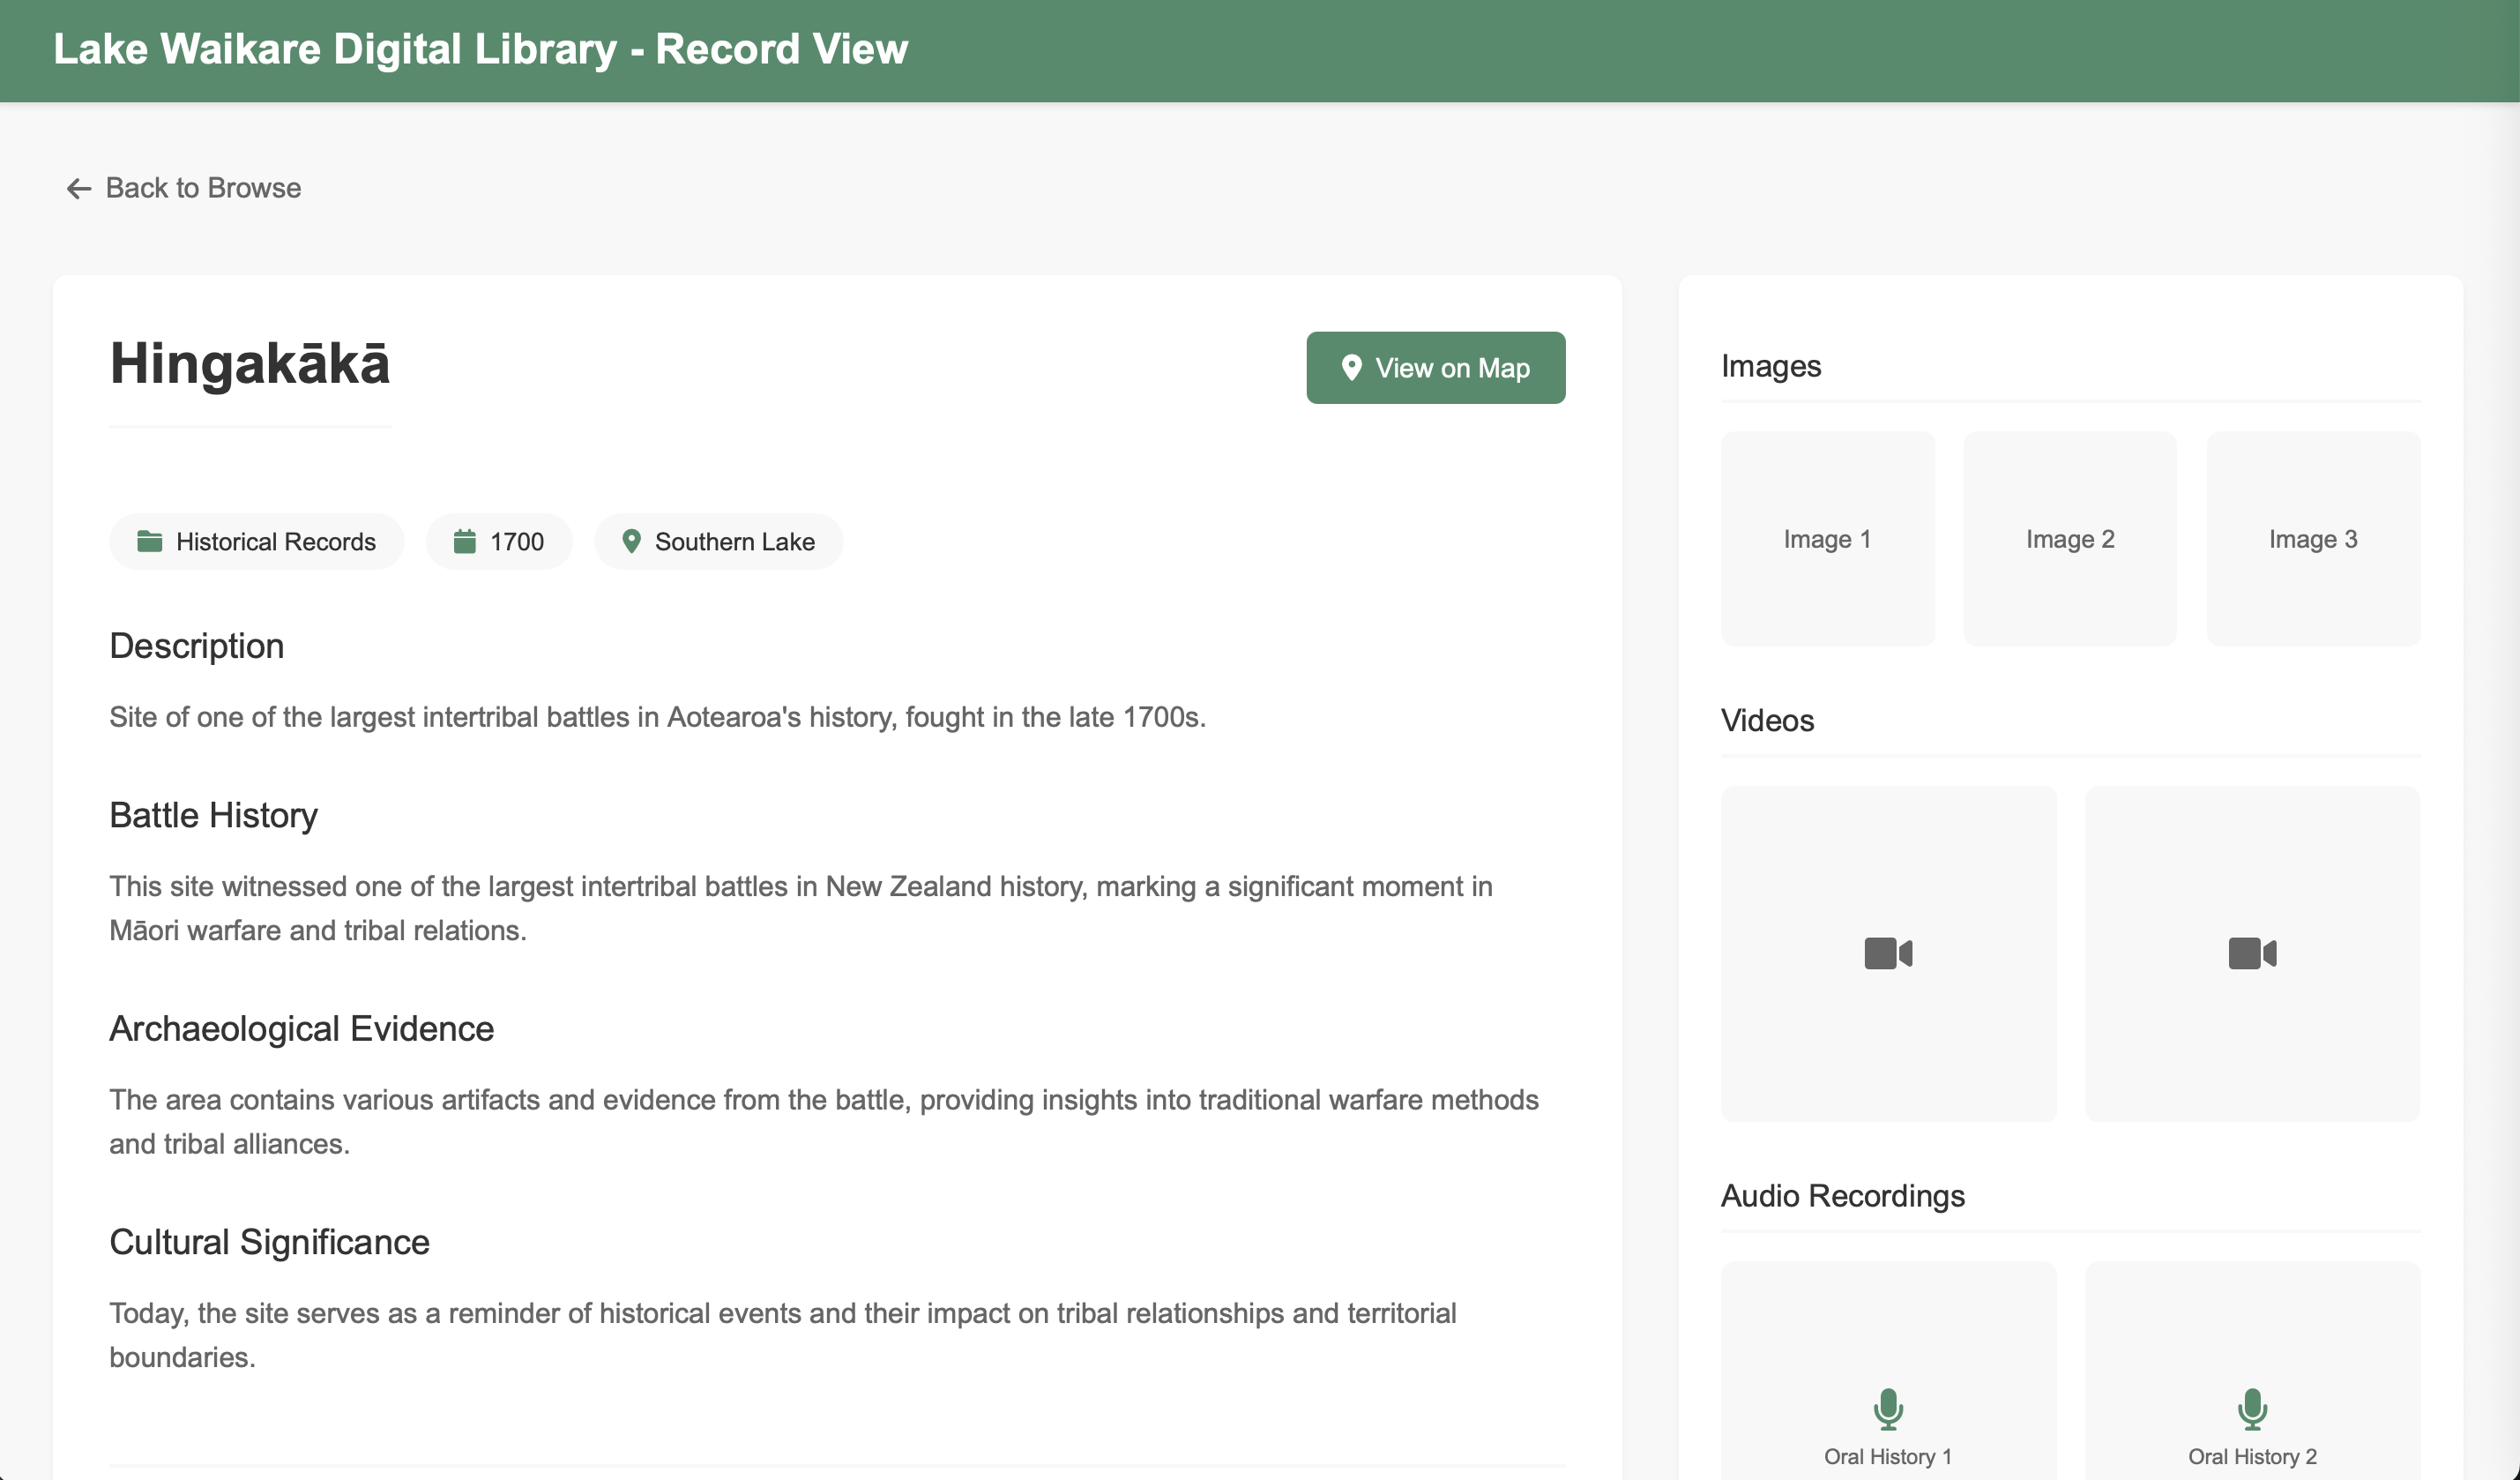
\includegraphics[width=0.8\textwidth]{screenshot/prototype_single_record.png}
    \caption{Single Record Page}
    \label{fig:architecture}
\end{figure}

The Record Detail Page can be accessed directly from the search results on the "Browse Records" page or by clicking on location markers on the map, allowing users to view detailed content from multiple entry points. At the top of the page, the record's title is prominently displayed, with clear information about the associated collection, relevant time period, and geographic location shown directly below. These details provide users with a comprehensive contextual framework to quickly understand the temporal and spatial background of the record.

To the right of the title, there is a prominent "Go to Map" button. When clicked, the page automatically navigates to the map view and centers on the specific location corresponding to the record. This feature greatly enhances the linkage between content and geography, enabling users to seamlessly transition from textual information to an intuitive geographic visualization, thereby improving overall interactive experience.

The main body of the page presents detailed core content of the record, structured clearly and written concisely yet informatively, helping users to deeply understand the specific details of the event or material. Below the main content, relevant supporting documents such as historical archives or battle records are provided as supplementary materials. These enrich the record's substance and meet the needs of users with varying levels of interest and research requirements.

On the right side of the page, there is a multimedia display area categorized into images, videos, and audio recordings related to the record. The image section showcases carefully selected historical photos or related artworks that visually represent the theme. The video section includes interviews, live footage, or explanatory clips that enhance the dynamic storytelling aspect. The audio recordings provide users with opportunities to listen to original audio materials such as traditional songs, oral histories, or lecture recordings. These multimedia elements not only elevate the visual and auditory richness of the page but also significantly enhance users' immersive experience.

The overall page design adheres to principles of clear information hierarchy, convenient interaction, and visual comfort. It ensures the content is both deep and authoritative while emphasizing smooth browsing and ease of use, aiming to create a comprehensive and engaging platform for exploring cultural heritage and historical information.

\subsection*{4.2.9 Admin Dashboard}
\addcontentsline{toc}{subsubsection}{4.2.9 Admin Dashboard}
\begin{figure}[H]
    \centering
    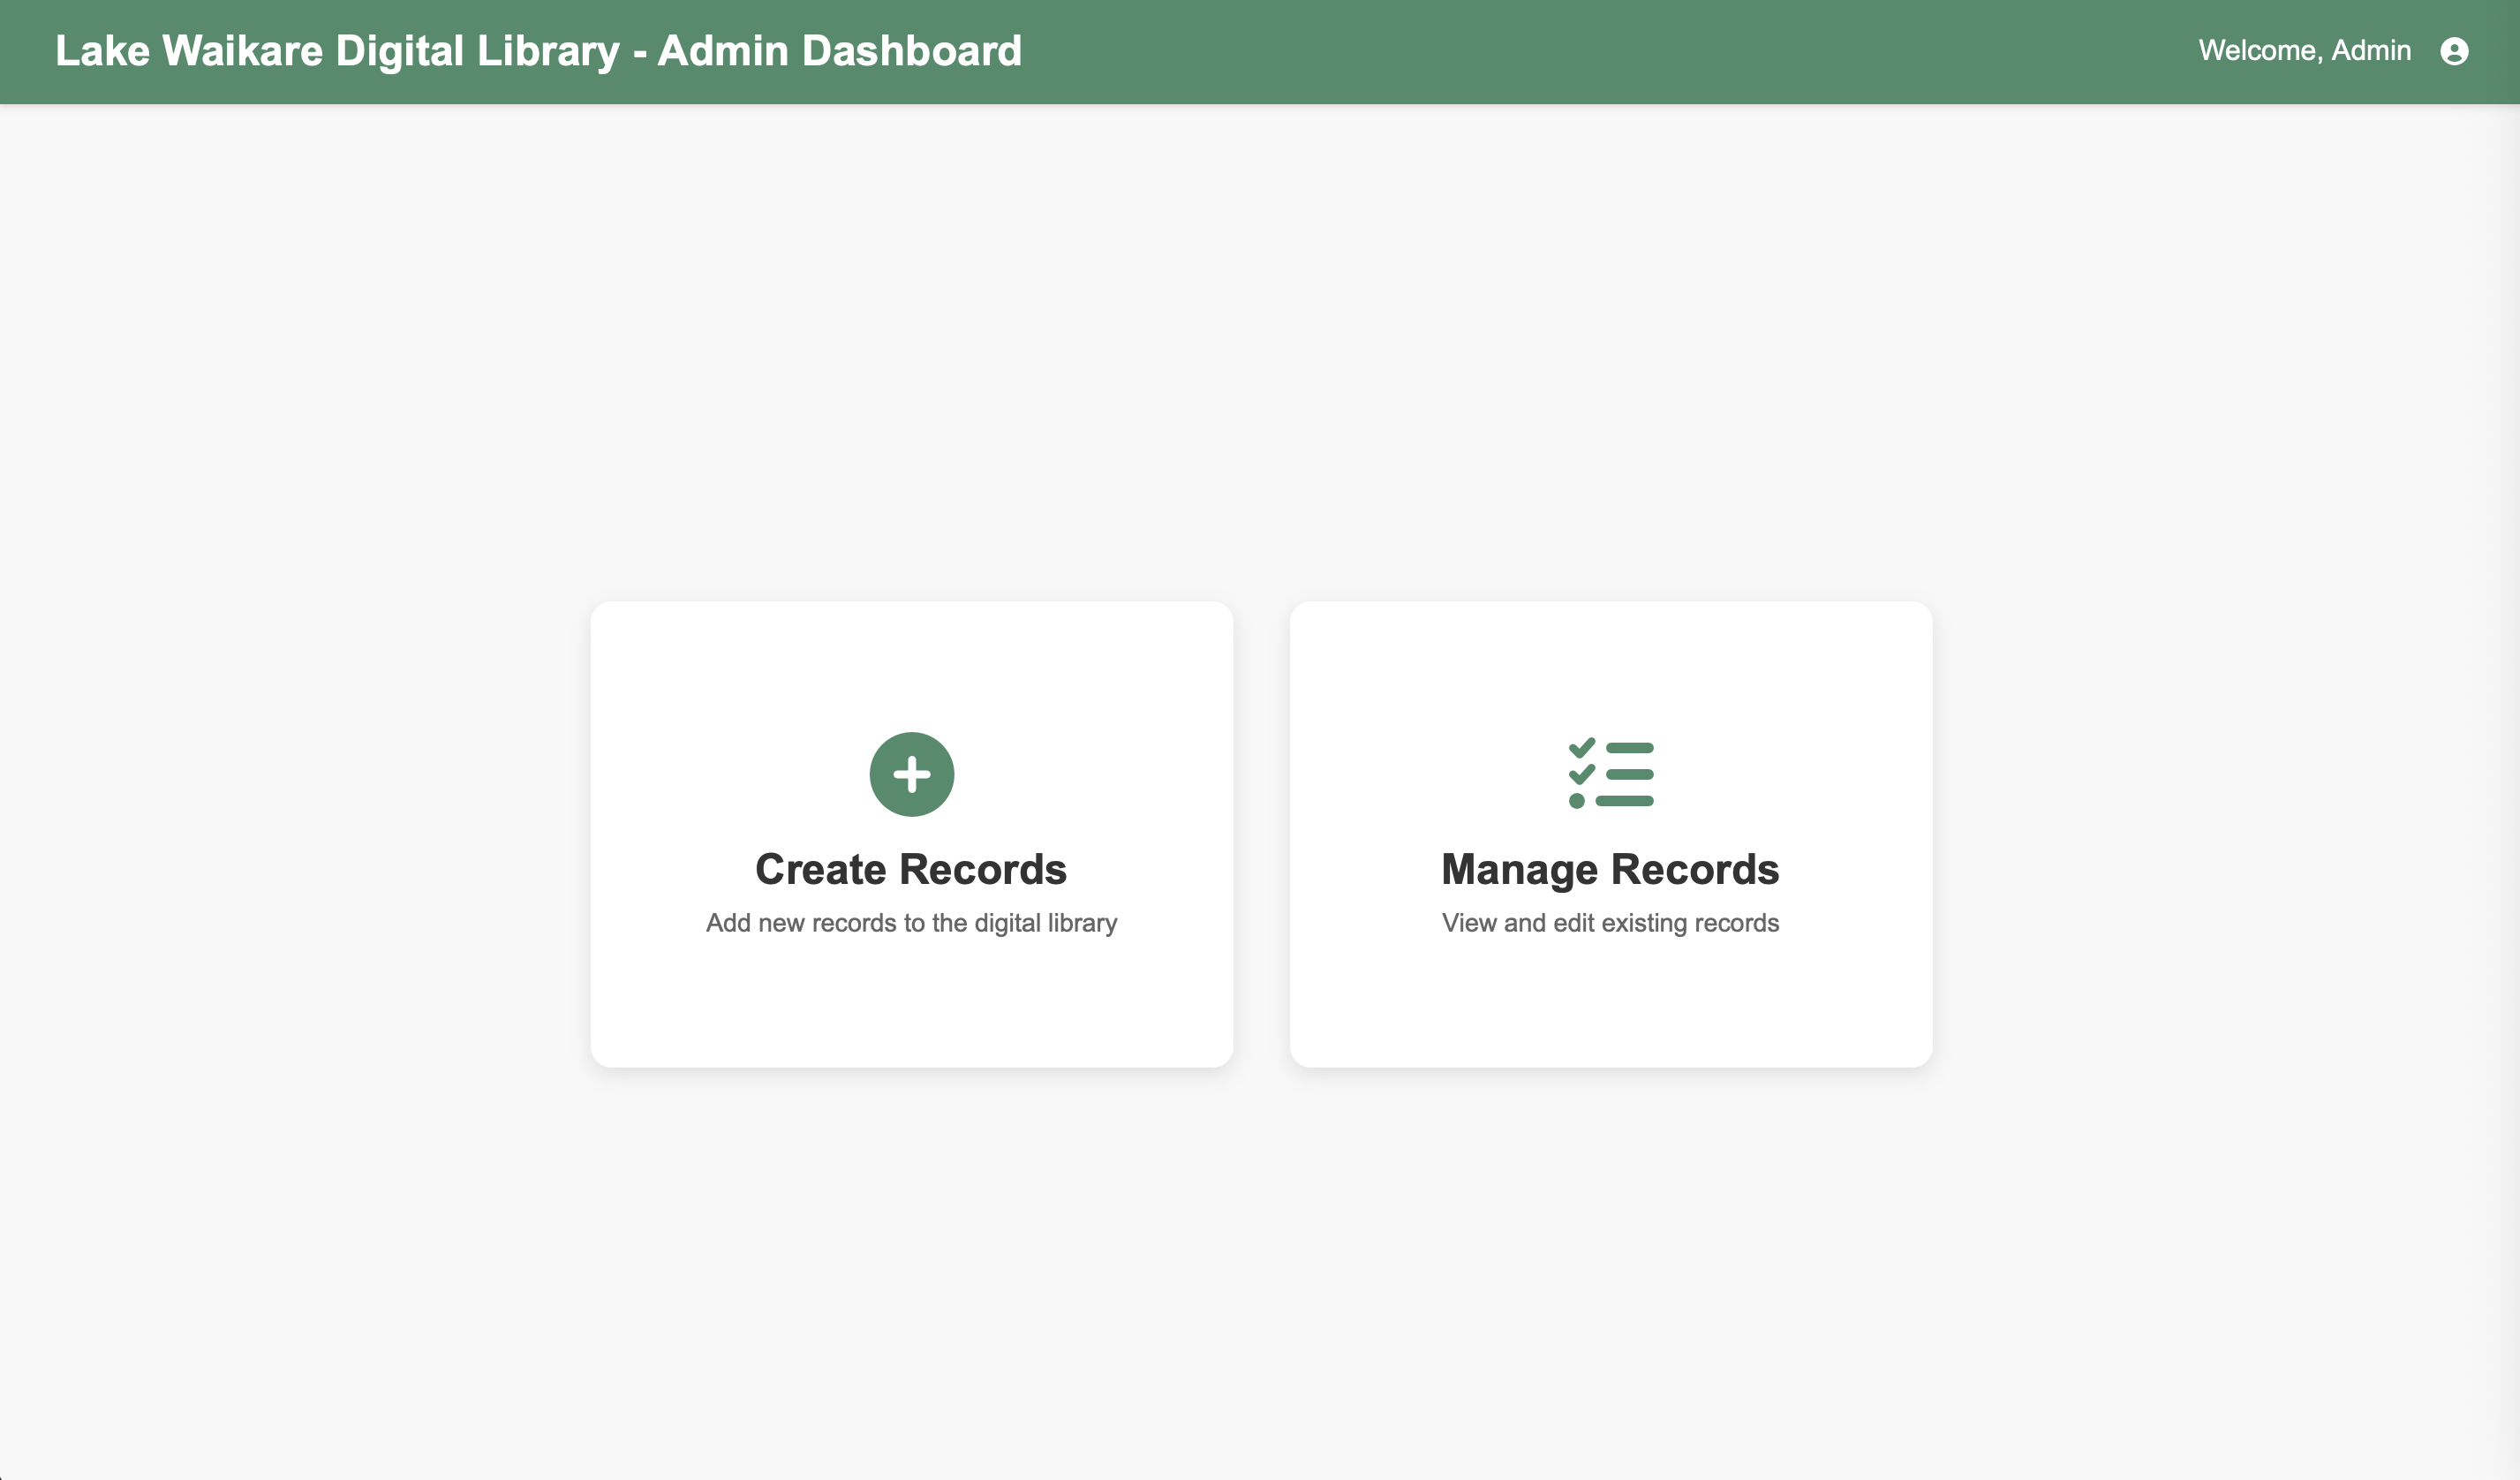
\includegraphics[width=0.8\textwidth]{screenshot/prototype_dashboard.png}
    \caption{Dashboard Page}
    \label{fig:architecture}
\end{figure}
The Admin Dashboard serves as a critical backend module for users with administrative permissions, enabling the creation, editing, and overall management of cultural records. This system supports the sustainable growth of content and ensures the integrity and accuracy of the cultural knowledge presented on the platform. Currently, the dashboard contains two key functions: record creation and record management. Together, these features support a complete workflow for content governance.

\begin{figure}[H]
    \centering
    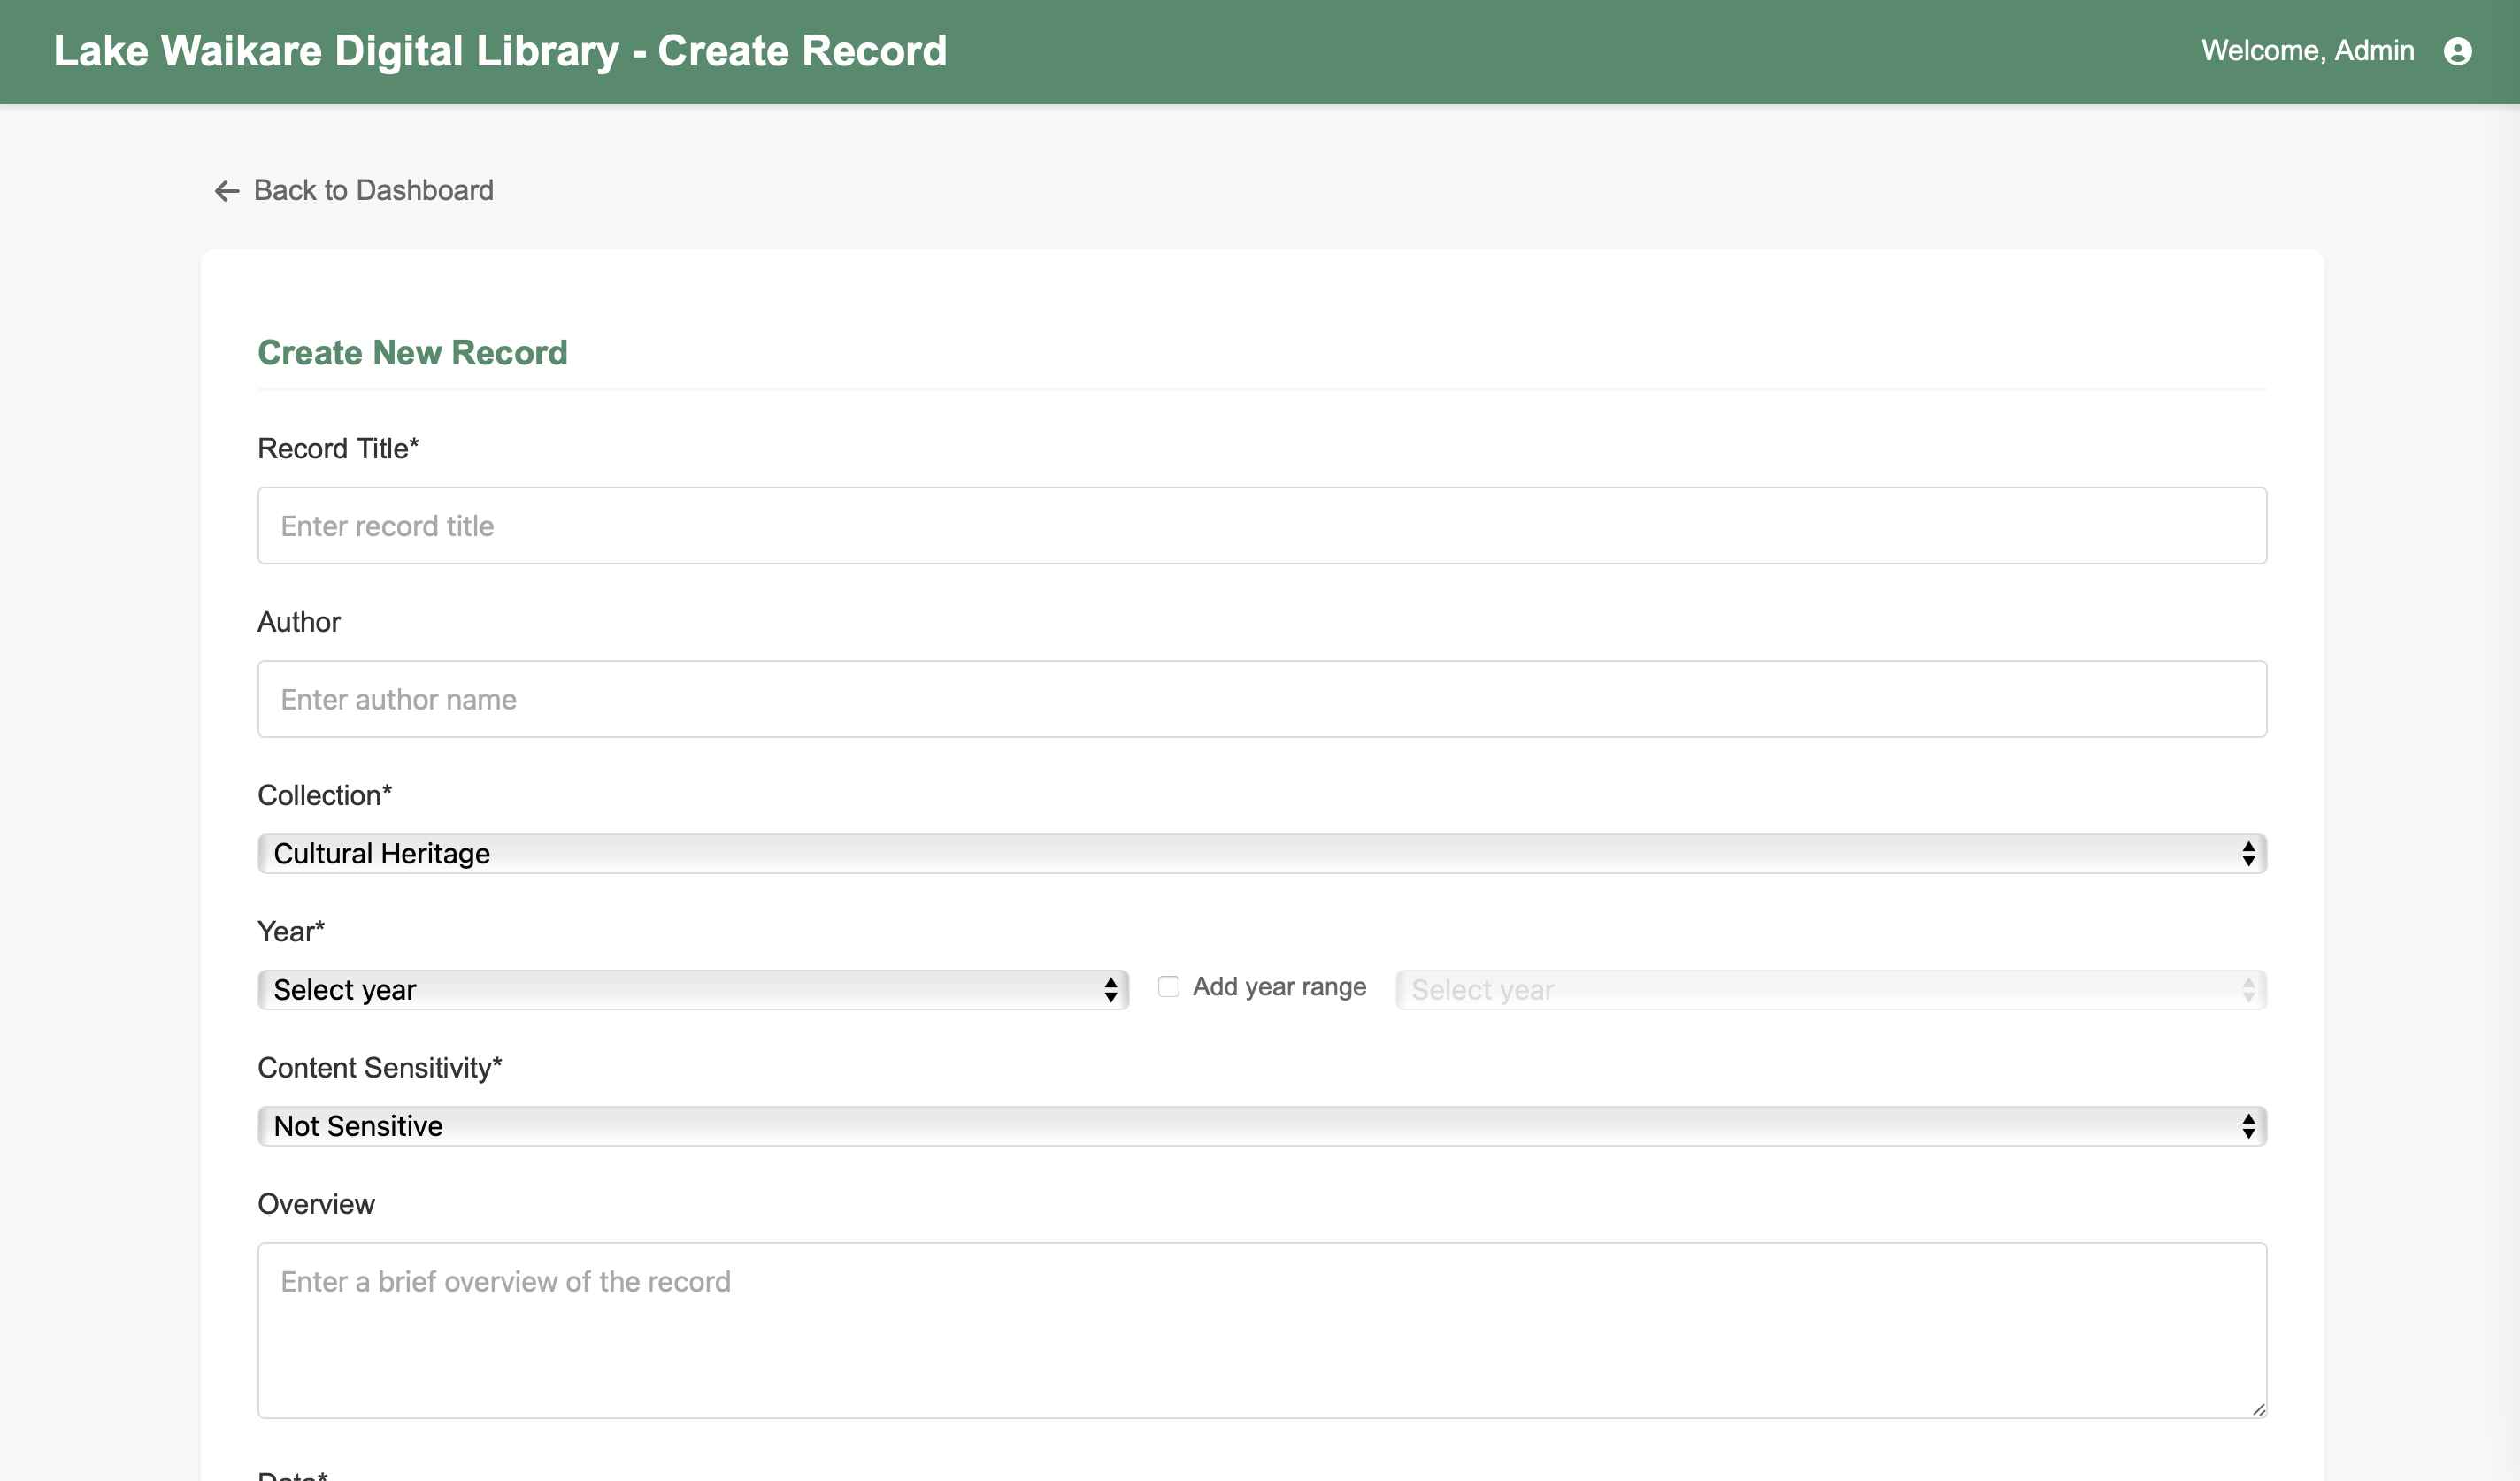
\includegraphics[width=0.8\textwidth]{screenshot/prototype_dashboard_createrecord.png}
    \caption{Dashboard Record Create Page}
    \label{fig:architecture}
\end{figure}
In the record creation page, administrators can input a new cultural record using a structured form that collects essential information such as the record title, author, collection name, and time period. The time input allows for both precise dates and flexible time ranges to accommodate records that may lack exact temporal references. An important feature of this interface is the ability to mark whether the content is considered sensitive. Sensitive records are only accessible to specific groups with appropriate permissions, a mechanism that helps protect Indigenous knowledge from inappropriate or unauthorized use. As part of this access control strategy, the system integrates Traditional Knowledge (TK) Labels. These labels provide culturally respectful indicators regarding how the record should be accessed or shared. For example, a TK label may restrict a record's visibility to members of a particular iwi or clarify that certain content should not be widely distributed. By embedding TK Labels into the metadata structure, the system aligns with principles of Indigenous data sovereignty and supports ethical content management practices.

To enrich the cultural record, the creation interface also supports uploading associated media such as documents, images, videos, and audio recordings. Each of these media types can be individually linked to the record, enhancing its narrative and educational value. In terms of spatial data, administrators can add a location to the record by clicking a map interaction button. This opens a dialog with a visual map, where users can drop a pin to define the exact geographic location, automatically capturing the latitude and longitude for future use within the map-based interface. At the bottom of the page, users are given the option to preview the record, save it as a draft, or publish it directly, depending on the stage of the editorial workflow.

\begin{figure}[H]
    \centering
    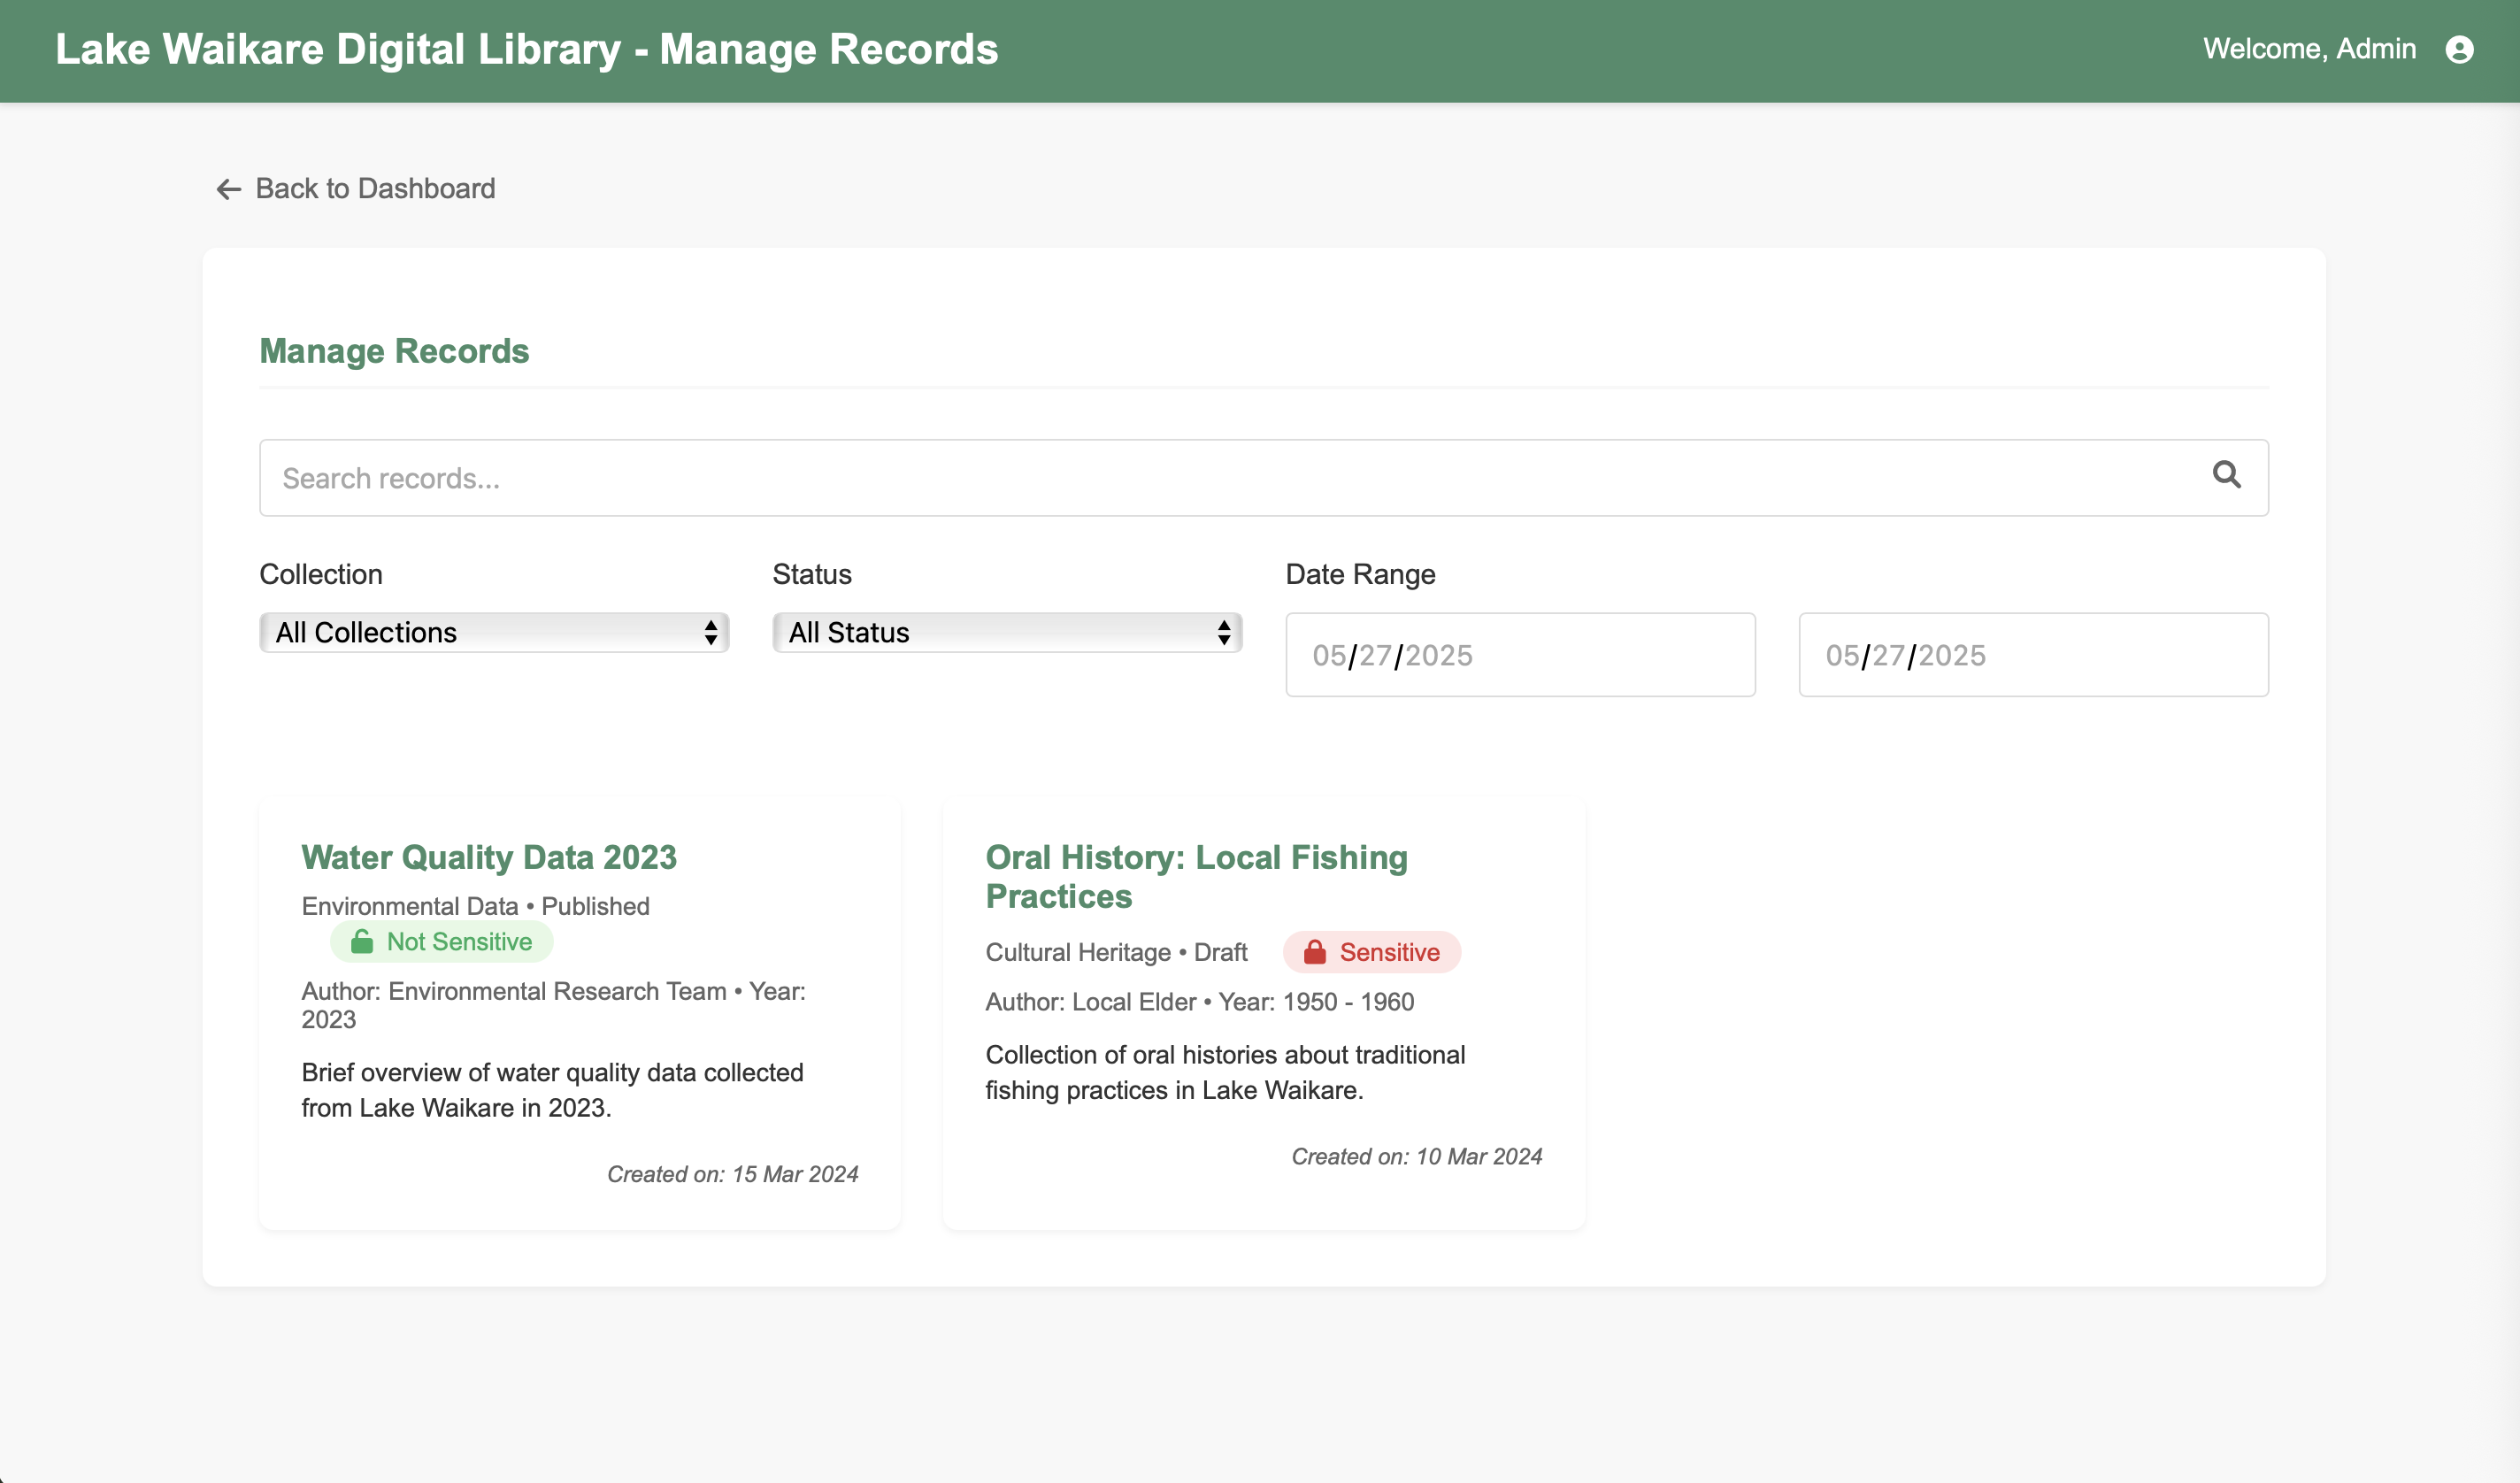
\includegraphics[width=0.8\textwidth]{screenshot/prototype_dashboard_managerecord.png}
    \caption{Dashboard Record Manager Page}
    \label{fig:architecture}
\end{figure}
The record management page allows administrators to review, update, or delete existing entries. It provides a search interface with multiple filtering options, including title, content, collection, status, and date range. This functionality allows for efficient retrieval of records, especially as the dataset grows in volume. When viewing a specific record from the list, a dialog window displays the record's full metadata, which can be edited. After editing, users can preview the changes, cancel the update, delete the record, or save the modification. The design of the interface supports intuitive operation while ensuring data integrity and minimizing the risk of accidental changes.

To support long-term preservation and structured organization of cultural materials, the platform will integrate Greenstone as its data repository. Developed by the University of Waikato in New Zealand, Greenstone is an open-source digital library system well-suited for managing multilingual, multimedia, and culturally significant content. Its robust metadata management, full-text indexing, and cross-format compatibility make it an ideal choice for storing and accessing Indigenous knowledge. By leveraging Greenstone, the platform ensures the durability of its digital archive and lays the groundwork for future interoperability and scholarly research.

In summary, the Admin Dashboard is not only the operational center for content entry and maintenance, but also a vital instrument in supporting cultural protection, respecting Indigenous knowledge rights, and promoting long-term digital stewardship. Through its implementation of TK Labels and its integration with Greenstone, the system builds a bridge between technology and cultural ethics, offering a powerful foundation for both community engagement and academic exploration.
